% This is the Reed College LaTeX thesis template. Most of the work
% for the document class was done by Sam Noble (SN), as well as this
% template. Later comments etc. by Ben Salzberg (BTS). Additional
% restructuring and APA support by Jess Youngberg (JY).
% Your comments and suggestions are more than welcome; please email
% them to cus@reed.edu
%
% See http://web.reed.edu/cis/help/latex.html for help. There are a
% great bunch of help pages there, with notes on
% getting started, bibtex, etc. Go there and read it if you're not
% already familiar with LaTeX.
%
% Any line that starts with a percent symbol is a comment.
% They won't show up in the document, and are useful for notes
% to yourself and explaining commands.
% Commenting also removes a line from the document;
% very handy for troubleshooting problems. -BTS

% As far as I know, this follows the requirements laid out in
% the 2002-2003 Senior Handbook. Ask a librarian to check the
% document before binding. -SN

%%
%% Preamble
%%
% \documentclass{<something>} must begin each LaTeX document
\documentclass[12pt,twoside]{reedthesis}
% Packages are extensions to the basic LaTeX functions. Whatever you
% want to typeset, there is probably a package out there for it.
% Chemistry (chemtex), screenplays, you name it.
% Check out CTAN to see: http://www.ctan.org/
%%
\usepackage{graphicx,latexsym}
\usepackage{amsmath}
\usepackage{amssymb,amsthm}
\usepackage{longtable,booktabs,setspace}
\usepackage{chemarr} %% Useful for one reaction arrow, useless if you're not a chem major
\usepackage[hyphens]{url}
% Added by CII
\usepackage{hyperref}
\usepackage{lmodern}
% End of CII addition
\usepackage{rotating}

% Next line commented out by CII
%%% \usepackage{natbib}
% Comment out the natbib line above and uncomment the following two lines to use the new 
% biblatex-chicago style, for Chicago A. Also make some changes at the end where the 
% bibliography is included. 
%\usepackage{biblatex-chicago}
%\bibliography{thesis}


% Added by CII (Thanks, Hadley!)
% Use ref for internal links
\renewcommand{\hyperref}[2][???]{\autoref{#1}}
\def\chapterautorefname{Chapter}
\def\sectionautorefname{Section}
\def\subsectionautorefname{Subsection}
% End of CII addition

% Added by CII 
\usepackage{caption}
\captionsetup{width=5in}
% End of CII addition

% \usepackage{times} % other fonts are available like times, bookman, charter, palatino


% To pass between YAML and LaTeX the dollar signs are added by CII
\title{Turnout and Mail Voting in Colorado}
\author{Theodore Dounias}
% The month and year that you submit your FINAL draft TO THE LIBRARY (May or December)
\date{December 2018}
\division{Mathematics and Natural Sciences and History and Social Sciences}
\advisor{Andrew Bray}
%If you have two advisors for some reason, you can use the following
% Uncommented out by CII
\altadvisor{Paul Gronke} 
% End of CII addition

%%% Remember to use the correct department!
\department{Mathematics and Political Science}
% if you're writing a thesis in an interdisciplinary major,
% uncomment the line below and change the text as appropriate.
% check the Senior Handbook if unsure.
%\thedivisionof{The Established Interdisciplinary Committee for}
% if you want the approval page to say "Approved for the Committee",
% uncomment the next line
%\approvedforthe{Committee}

% Added by CII
%%% Copied from knitr
%% maxwidth is the original width if it's less than linewidth
%% otherwise use linewidth (to make sure the graphics do not exceed the margin)
\makeatletter
\def\maxwidth{ %
  \ifdim\Gin@nat@width>\linewidth
    \linewidth
  \else
    \Gin@nat@width
  \fi
}
\makeatother

\renewcommand{\contentsname}{Table of Contents}
% End of CII addition

\setlength{\parskip}{0pt}

% Added by CII

\providecommand{\tightlist}{%
  \setlength{\itemsep}{0pt}\setlength{\parskip}{0pt}}

\Acknowledgements{

}

\Dedication{

}

\Preface{
This is an example of a thesis setup to use the reed thesis document
class.
}

\Abstract{

}

% End of CII addition
%%
%% End Preamble
%%
%

\begin{document}

% Everything below added by CII
      \maketitle
  
  \frontmatter % this stuff will be roman-numbered
  \pagestyle{empty} % this removes page numbers from the frontmatter

  
      \begin{preface}
      This is an example of a thesis setup to use the reed thesis document
      class.
    \end{preface}
  
      \hypersetup{linkcolor=black}
    \setcounter{tocdepth}{3}
    \tableofcontents
  
      \listoftables
  
      \listoffigures
  
  
  
  \mainmatter % here the regular arabic numbering starts
  \pagestyle{fancyplain} % turns page numbering back on

  \chapter*{Introduction}\label{introduction}
  \addcontentsline{toc}{chapter}{Introduction}
  
  The democratic system is based on procedures as much as principles. The
  way that democracies chose to tally the will of the people is always a
  messy, controversial process. Thus the design and implementation of
  voting systems is far from being neutral; the decisions made on who
  votes, and how, when, and where they do so is inherently coupled with
  the outcome. Underlying those decisions is a nebulous, inconclusively
  answered question: are elections fair, and how can we make them more so.
  
  The passage of the Help America Vote Act---or HAVA--(Robert Nay, 2002),
  which mandated states to update and consolidate public voter
  registration files, and created the US Elections Assistance Commission
  that makes available county level data, innovated the way we use data
  based approaches to answer this question. HAVA offered political
  scientists and statisticians direct access to the voting population's
  voting patterns, political registration, age, geolocation and much more;
  information that up to then was only accessible by sampling through
  surveys. The immense leap here happens because true population data does
  away with the need for sampling techniques that are often biased and
  inaccurate. We can now not only get a complete picture of the data, but
  also link and merge with other sources of information such as US Census
  data on religion, race, education, or income---work that has been
  lucrative for firms such as Catalist or Target Smart. By posing
  Political Scientific questions, and trying to respond with rigorous
  statistics, both disciplines tackle these data to face joint problems
  such as quantifying the quality of voter registration files
  (Ansolabehere \& Hersh, 2010), or linking disparate voter records
  (Ansolabehere \& Hersh, 2017).
  
  \chapter{The State of the Literature}\label{rmd-basics}
  
  In this chapter I will go through the existing literature on
  Vote-By-Mail (VBM).I will first go through some general literature on
  theories of voting decisions. I will define what Vote-By-Mail is; I will
  then summarize the expectations that researchers have of the effects of
  VBM on turnout, based on existing theories of electoral participation. I
  will continue with a summary of previous quantitative research on the
  effects that VBM and similar policies have had on turnout. I will
  conclude with some more general comments on the available data, and
  literature concerning the most commonly used quantitative methods.
  
  \section{Deciding to Vote}\label{deciding-to-vote}
  
  \subsection{Why Turnout Matters}\label{why-turnout-matters}
  
  Turnout is the most commonly used measure for electoral participation.
  It is important because it signifies the level of engagement of the
  population with the state, the level of incorporation of different
  subgroups of the population into democratic processes, and the
  legitimacy of elected officials. It is widely accepted that turnout
  should be maximized so that the democratic franchise represents the
  majority of citizens. Turnout for an election can be calculated or
  predicted, the difference being that in the former case we use data
  post-election to measure its absolute value, while in the latter we use
  a series of individual and community covariates to infer the levels of
  turnout for a future or past election.
  
  Calculating turnout, at its core, involves the following equation:\\
  \[ \% ~Turnout = \frac{Total~Ballots~Cast}{Measure~of~Total~Voting~Population}\times100\%~~~(1)\]
  
  The choice of numerator is fairly obvious and universal; the
  denominator, however, is a different story. The two main statistics used
  are the total voting age population, and the raw number of registered
  voters in the geographical location we are examining. The total voting
  age population is used as a measure to incorporate the total amount of
  possible voters in a geographical area, and can be measured using data
  from the US Census. This causes some issues with voters that cross over
  to different districts; if someone lives in district A, it is still
  likely that they are registered to vote in district B. If this is not
  considered, the calculation of voting age population might be
  misrepresentative.
  
  Using registered voters also brings with it two problems. First, the
  calculation necessarily occurs using voter registration files, which
  many times can include discrepancies, like deceased voters, voters
  included in multiple counties, or individual voters included multiple
  times. Furthermore, the total amount of actual voters among registered
  voters can be misrepresentative of democratic participation; consider
  that if a certain minority community has historically low registration
  rates, their lack of engagement will not be included in turnout rates,
  thus misrepresenting the level of inclusion in the district they reside
  in.
  
  The punch line here is that how the turnout statistic is calculated is
  not a clear choice, and will have an impact on how studies are set up.
  To give one example, consider Oregon's Motor Voter program, that
  automatically registers voters when they interact with government
  services, like the DMV. It is conceivable that this reform will
  \emph{decrease} turnout when measured as a percentage of the total
  registered voter count, but \emph{increase} turnout when measured
  against total population. I will specify how I calculate turnout in the
  next chapter.
  
  Statistical models of turnout can be constructed at either the
  individual or community level. At the individual level, a model is built
  to predict the probability of voting for every member of a group, and
  then sum over the members to create an estimate for turnout. Probit or
  Logit models are preferred. At the community level, researchers first
  choose a geographical level at which to calculate, which then
  constitutes the individual observation in the data that is used to
  create the model.
  
  Both these models include a standard set of societal variables--at the
  individual and aggregate level--, policy variables--whether the district
  does Postal Voting, whether Voter ID requirements are particularly
  strict--, election-specific variables--closeness of election or campaign
  expenditure--and sometimes time-series data--previous levels of
  turnout--to make predictions on turnout levels. This type of analysis is
  not exclusively used to predict turnout but also to, as will be later
  shown, draw inferences on the effects that certain explanatory variables
  have on electoral participation.
  
  Through meta-analyses on studies of turnout, it is possible to get a
  clear picture on what variables effect individual and collective choices
  to turn out. Three such studies are conducted by Geys (2006), Geys and
  Cancela (2016), and Smets (2013). Geys includes 83 studies of national
  US elections in his initial meta-analysis (Geys, 2006), later increasing
  that number to 185 (Geys and Cancela, 2016) and adding local elections.
  On aggregate-level models for national elections they conclude that
  competitiveness, campaign financing, and registration policy have the
  most pronounced effects, while on the sub-national level there are more
  pronounced effects for societal variables and characteristics of
  election administration (spending, voting policy, etc.). Smets and Van
  Ham (2013) examine individual-level predictors for turnout in a similar
  meta-analysis, and conclude that ``age and age squared, education,
  residential mobility, region, media exposure, mobilization (partisan and
  nonpartisan), vote in previous election, party identification, political
  interest, and political knowledge'' (Smets \& Ham, 2013) are the most
  significant explanatory variables for turnout, along with income and
  race. I will specify the model I will use for turnout in the second
  chapter.
  
  \subsection{Theories of Voting}\label{theories-of-voting}
  
  Here I take one step back from turnout, and examine the theories
  surrounding individual choices to vote or abstain. There are three main
  theories outlined in the literature on why individuals chose to vote.
  While there is some overlap, the following are mostly distinct:
  
  \begin{itemize}
  \item
    \emph{Decision ``at the margins''}: In his 1993 study, Aldrich posits
    that voting is a low cost-low benefit behavior. Therefore, he
    continues, voting is a decision that individuals make ``at the
    margins''; in most people, the urge to vote is not overwhelmingly
    strong, and therefore individuals will vote when it is convenient to
    them, when they are motivated by a competitive race, when policies are
    put in place to help them, and when they are subjected to GOTV (Get
    Out the Vote) efforts. For Aldrich, this is corroborated by the fact
    that most turnout models present consistent, yet weak, relational
    variables; if decisions are made ``at the margins'', then no single
    predictor would have an overwhelming result. This is also supported by
    Matsusaka (1997), and Burden \& Neiheisel (2012). Matsusaka expresses
    support for a more ``random'' process of voting, where turnout models
    are ambiguous because of the difficulty that predicting ``at the
    margins'' entails (Matsusaka \& Palda, 1999). Burden \& Neiheisel
    (2013) also demonstrate support for Aldrich's thesis by using data
    from Wisconsin to calculate a net negative effect of 2\% on turnout
    due to a similar slight shift in turnout.(Aldrich, 1993; Neiheisel \&
    Burden, 2012)
  \item
    \emph{Habitual Voting}: While Aldrich supports that there is no single
    overwhelming predictor of turnout, Fowler (2006) posits that future
    voting behavior can be strongly predicted using individual voting
    history. This leads to the conclusion that individuals are set to
    either be habitual voters, or habitual non-voters (Plutzer, 2002) by
    their upbringing and social circumstances, locking them into distinct
    groups. (Fowler, 2006)
  \item
    \emph{Social/Structural Voting}: Close to habitual voting are those
    that support a model of social and structural voting; these
    researchers claim that the decision to vote or not is deeply rooted in
    socioeconomic factors, which means that the divide between
    traditionally voting and non-voting groups can only be bridged by
    directly dealing with the socioeconomic divide between them (Berinsky,
    2005; Edlin, Gelman, \& Kaplan, 2007 ). Their reasoning is that ``at
    the margins'' voting only addresses groups that do not face
    significant burdens against voting--like the working poor, or
    marginalized racial groups--, and are usually already registered.
    Similarly, they address habitual voting claims by arguing that they
    are too short-sighted; individuals themselves might be habitually
    voting, but their decision to do so is rooted in strong societal and
    policy factors.
  \end{itemize}
  
  \section{From Theory to Policy}\label{from-theory-to-policy}
  
  \subsection{Voting Styles}\label{voting-styles}
  
  I have already flagged in my introduction the reason why theories behind
  voting choice matter: each construct an image of the electorate that
  reacts differently to policy change around voting. They are all an
  answer to the fact that voting policy, and how we conduct elections, is
  not value neutral but has implications for turnout, which in turn has
  implications on the franchise of democracy.
  
  In trying to respond to the issues set up by theoretical paradigms,
  different states--both in the world and US contexts--have adapted to
  different ways of conducting elections. In the US, voting styles can be
  simplified into three categories:
  
  \begin{itemize}
  \item
    \emph{In-Person Election Day}, for which all individuals are required
    to vote at a polling place, on a single election day. There can be
    some leeway for overseas voters, or excused absentee voters, but the
    vast majority of people will have to be present to vote in a
    particular time frame.
  \item
    \emph{In-Person Early Voting}, for which all individuals must vote in
    person at a polling place or vote center, but the timeframe for voting
    extends for around two weeks, not a single day.
  \item
    \emph{Vote-By-Mail, Absentee Early Voting}, for which individuals have
    a clear, no-excuse-necessary option for not being present when they
    vote, or for filing in a mailed ballot and droping it off at
    designated locations.
  \end{itemize}
  
  For the purposes of this thesis I will examine the latter category, and
  specifically Vote-By-Mail. The reason behind this is that the model of
  in-person, election day voting is usually seen as the baseline, the
  ``vanilla'' way of conducting elecions if you will. Therefore it has
  been of interest for researchers to examine if other systems can
  outperform that baseline. Specifically, it is most interesting to
  examine voting styles that are heralded for their expansion of turnout,
  to see whether popular beliefs on their benefits and drawbacks hold; if
  they are different from the base model of conducting American elections,
  or if they present new challenges and unique selling points.
  Vote-By-Mail is particularly intersting because it is quickly taking the
  form of a trend in state elections, as more and more states are
  enforcing more open models of VBM. In the next section, I will more
  closely examine the particulars of Vote-By-Mail.
  
  \subsection{What is VBM?}\label{what-is-vbm}
  
  Vote-By-Mail is a process by which voters receive a ballot delivered by
  mail to their homes. Voters then have a variety of options on how to
  return these ballots, ranging from dropping them off at pre-designated
  locations, to mailing them in, to bringing them to a polling place and
  voting conventionally. This varies across states that have implemented
  VBM. Some common forms of the VBM policy are:
  
  \begin{itemize}
  \tightlist
  \item
    \emph{Postal Voting}: All voters receive a ballot by mail, which can
    then be returned to a pre-designated location or mailed in to be
    counted. This is the current system in Oregon, is an option in
    Colorado, and is implemented by a number of counties in California,
    Utah, and Montana.\\
  \item
    \emph{No-Excuse Absentee}: Voters can choose to register as absentee
    voters without giving any reason related to disability, health,
    distance to polling place etc. This is the case in 27 states and the
    District of Columbia.\\
  \item
    \emph{Permanent No-Excuse Absentee}: This is similar to the previous
    system, but allows voters to register as absentees indefinitely,
    without having to renew their registration each year; they become de
    facto all-mail voters. This is in place in Washington, Kansas, and New
    Jersey.\\
  \item
    \emph{Hybrid or Transitionary Systems}: In hybrid systems, voters
    receive a mail ballot but can choose to disregard it and vote
    conventionally. This is the case in Colorado. Transitional systems
    exist in states that have chosen to eventually conduct all elections
    by postal voting, but have given counties an adjustment period during
    which this shift is not mandatory, or mandatory only for certain
    elections. This is the case in California, Utah, and Montana.
  \end{itemize}
  
  Vote-By-Mail is also commonly considered a type of early voting, since
  voters receive their ballots around two weeks in advance of election
  day; they are also able to return that ballot whenever they wish within
  that time-frame. This means that Vote-By-Mail can be counted as a
  ``convenience voting'' reform. These are usually implemented by state
  and local governments with the argument that they either expand the
  democratic franchise by bringing in new voters, or by making it more
  likely that current registered voters participate in the electoral
  process.
  
  \subsection{How Theories Apply to VBM}\label{how-theories-apply-to-vbm}
  
  Under Aldrich's paradigm, vote by mail would not effect significant
  change in voting behaviour. The whole concept of a decision ``at the
  margins'' is that the forces at play when an individual decides to vote
  are overwhelmingly strong both ways, so any effect that policy can have
  will minimaly shift these margins. If, for example, we take a
  presidential eleciton the forces at play include the media, national
  committees, social effects etc. In this environment some added
  convenience does not significantly add to an individual's decision to
  turn out. However, this would indicate that at a local level, where
  national and media effects are less strong, the effect of VBM on turnout
  might be more significant. The effect would be present for all groups,
  not only those currently registered, since voting would be easier
  uniformly.
  
  If we asume habitual voting, the conclusion on VBM would differ
  significantly. In this case, the effect to be considered is how VBM
  impacts already formed habits around voting. It could be argued that VBM
  has no effect, which follows if we assume that voting habits formed do
  not shift if the mode of voting changes. It could also be argued that
  VBM might have a negative effect on turnout in the short term, because
  it disrupts the habit of election day for a readjustment period, before
  people settle into new groups of habitual voters and non-voters, adapted
  to the new policy context.
  
  Under social and structural voting contexts, VBM retains rather than
  stimulates new voters (Berinsky, 2005). This means that already
  registered and semi-active voters are more likely to participate, but
  there is no significant change in the amount of new voters entering the
  franchise. This would mean that traditional forms of voting policy that
  emphasize access to the polls will do nothing to bring in
  disenfranchised people, and potentially hide the problem under an
  inflated turnout statistic calculated on registered voters. Berinsky in
  particular emphasizes the need for a shift towards voter education,
  rather than early voting or VBM policies (Berinsky, 2005).
  
  \section{Previous Study Results}\label{previous-study-results}
  
  In this section I will go through previous results from studies of
  Vote-By-Mail. I will also include a series of studies that are not
  necessarily about VBM, but have either been conducted in Vote-By-Mail
  states, or have to do with early voting which, as I have mentioned, is
  frequently linked to VBM. Most studies include a set of models or
  predictions of turnout, which are split into individual or county level
  results. I will group the studies according to whether the result shows
  a negative or positive effect on turnout.
  
  \subsection{General Results on VBM}\label{general-results-on-vbm}
  
  I will start with studies that show a negative effect on turnout.
  Bergman (2011) uses a series of logit models of individual voting
  probability in California, during a period where part of the state
  conducted VBM elections, while others maintained traditional voting.
  This is called a ``quasi-experiment'', and is frequent throughout the
  literature. Bergman's results show a statistically significant drop in
  voting probability in VBM counties (Bergman \& Yates, 2011). Using a
  similar method, Keele (2018) takes a single city in Colorado, Basalt
  City, which is divided into two different voting districts using
  different voting systems. The conclusion is, again, a 2-4\% drop in
  turnout along the VBM part of the city (Keele \& Titiunik, 2017). Burden
  et al. (2014) takes a different approach, using country-wide election
  data from 2004 and 2008 presidential elections, and compares districts
  based on early voing practices. Their results show a significant drop in
  turnout, which can be associated to VBM as well due to its closeness to
  EV (Burden, Canon, Mayer, \& Moynihan, 2014).
  
  In contrast, Gerber et al. (2013), applying both individual and
  county-level models for the state of Washington, reach the conclusion
  that VBM increases turnout by around 2-4\%; they use the same
  quasi-experimental model that offers itself to researchers in states
  that are under transitionary systems (Gerber, Huber, \& Hill, 2013).
  R.M. Stein also reaches a similar conclusion when examining Colorado's
  practice of ``vote centers'', which are non-precinct attached polling
  places, which can service multiple counties (Stein \& Vonnahme, 2008). I
  include this paper here due to the link that voting centers have with
  VBM, as they serve as drop-off points for mail-in ballots. Richey (2008)
  examines the effects that Oregon's VBM program has on turnout by using
  past elections data, concluding a 10\% positive trend associated with
  the policy (Richey Sean, 2008). This effect is studied again by Gronke
  et al.(2012) who find a similar positive effect with much lower
  magnitude, which might point to a novelty effect: the existence of
  diminishing returns in turnout after the implementation of this policy
  (Gronke \& Miller, 2012). Gronke et al. (2017), again studying Oregon
  but focusing on Oregon's Motor Voter program, find evidence of positive
  association to turnout {[}@{]}. I include these effects due to Oregon
  being an exclusively VBM state, and because this paper uses a
  ``synthetic control group'' model, a particularly interesting
  statistical technique. Lastly, I include a study conducted by Pantheon
  Analytics on Colorado, which compares actual turnout to predicted levels
  for VBM counties in Colorado. The results show a positive effect of
  approximately 3.3\% due to VBM (Edelman \& Glastris, 2018).
  
  The conclusion to be drawn from this section is that results on VBM vary
  significantly. There are multiple studies, using multiple methods, on
  multiple states, with multiple results. This only adds to the importance
  of being careful when constructing models and hypotheses to test VBM's
  effects on turnout, as assumptions made in the process can critically
  impact the results.
  
  \section{Voter Registration Files}\label{voter-registration-files}
  
  \subsection{Inaccuracy of Survey Data}\label{inaccuracy-of-survey-data}
  
  Apart from Voter Registration Files, the main source of data on the
  American electorate is national surveys, like the American NAtional
  Election Studies' survey (ANES), or the Cooperative Congressional
  Elections Study (CCES). These are post-election surveys, distributed to
  voters, which include fields associated directly with
  voting--participation, precinct, which party you voted for--and
  indirectly, through questions on societal factors like race, income, or
  gender. On the surface these seem like a better source of data, since no
  record linkage or ecological inference need be made to connect
  individual voters with an extensive list of covariates. There is,
  however, a significant problem with these data: survey misreporting.
  
  Even without resorting to advanced statistical or data gathering
  methods, the fact that the CCES and NES often misrepresent the
  electorate is apparent just through looking at turnout statistics; both
  show higher turnout than what the true value, calculated from the
  population, was. When looking at surveys a bit closer, using either
  private, extensive data files like Catalyst (Ansolabehere \& Hersh,
  2012) or validated voter files from the late 20th century (Deufel \&
  Kedar, 2010), the results show consistent misreporting among certain
  groups, that tend to either be politically engaged non-voters or
  minorities and low socioeconomic status individuals. This gap, according
  to Deufel et al. (2010), has served to propagate societal stereotypes
  and class entrenchment into studies on turnout, which in turn
  negativelly effect policy, since research using the ANES and CCES are
  widely used to study turnout among the groups that are consistently
  misreporting. Admittedly, the fact that misreporting happens among
  specific groups does open the way for statistical methods to compensate
  for the bias intoduced, but for the purpose of my thesis I will prefer
  the use of VRF.
  
  A last issue with surveys worth mentioning is that they are contingent
  on quantity of responses as well as quality. There is no guarantee that
  the CCES or NES will receive enough responses to correctly infer
  population-wide statistics; something which is more likelly for the
  American Community Survey or the Census, whcih are backed by the
  legitimacy of the federal government. Survey under-reporting is directly
  linked with the practices of the groups conducting the survey, and as
  such is hard to control for after the results are published (Burden,
  2000).
  
  \subsection{The Importance of VRF}\label{the-importance-of-vrf}
  
  As mentioned in my introduction, access to voter registration files has
  provided researchers with unique insight into the voting process.
  Quantitative research has expanded significantly, for three key reasons.
  First, VRF data exists in a consolidated, state-wide format at least for
  national elections. This means that the process of data collection
  involves interaction with significantly fewer government agencies, and a
  data wrangling process that can be quickly adapted to a set format. This
  is, of course, not to say that the process of data collection and
  handling doesn't still pose a significant challenge, as will become
  apparent in my second chapter. Second, there is a huge benefit attached
  to the fact that VRF data describes the whole population, rather than a
  sample. As mentioned in the previous section, survey data might give
  more insight into variables not included in VRF, but that comes at a
  steep cost for accuracy. Using VRF, the problem of self-reporting bias
  is eliminated for some studies, and transformed into a problem of record
  linkage and ecological inference for others (Ansolabehere \& Hersh,
  2017, Burden \& Kimball (1998)). Third, wide public access means
  reproducibility and accessibility, which translates into greater
  accountability for researchers. This effect is important, even if
  mitigated somewhat by private data companies and access fees.
  
  \section{Common Methods Used and Problems
  Encountered}\label{common-methods-used-and-problems-encountered}
  
  \subsection{Methods}\label{methods}
  
  \begin{itemize}
  \tightlist
  \item
    \emph{Synthetic Control Group}: Abadie (2010), McClleland (2017),
    Gronke (2017)
  \item
    \emph{Record Linkage}: Ansolabehere and Hersch (2017), Harvey (1994,
    97), Koudas (2013)
  \item
    \emph{GLM (Probit/Logit/Poisson)}: Barreto (2004), Dow (2004)
  \item
    \emph{DID}: Bertrand et al. (2002)
  \item
    \emph{E.I.}: King (2013), Burden (1998), Calvo (2003), Chao (2004), Rm
    Stein (2002)
  \item
    \emph{Mixed-Effects}: Gelman and Hill (2007)
  \item
    \emph{General EDA and Models}: James et al. (2013), Chapman and Hall
    (2017)
  \end{itemize}
  
  \chapter{Hypotheses and Methods}\label{hypotheses-and-methods}
  
  In this chapter, I introduce a series of questions resulting from the
  literature review of Chapter 1, which I will use to formulate
  hypotheses. I will then operationalize these hypotheses, and attempt to
  predict analytical outcomes based on the theories of Chapter 1.
  Following these hypotheses, I will outline key methods I will use to
  test them.
  
  \section{Hypotheses}\label{hypotheses}
  
  \subsection{Questions}\label{questions}
  
  Before moving in to outlining hypotheses, the first step necessary is to
  frame a series of questions, which the hypotheses will flow from. Based
  on relevant research, the most obvious first question to ask would be:
  
  \[Q1: What~is~the~effect~of~mail~voting~on~turnout? \]
  
  I went through this question substantially in the previous chapter; it
  should be clear that depending on which paradigm of participation choice
  is present, the answer here can be radically different.
  
  In order to best answer the previous question, it is necessary to
  establish some conditions on importance of effect. Therefore it is also
  necessary to ask the following question:
  
  \[Q2: Is ~this~ effect~ significant ~when~ compared~ to ~other~ metrics~ that~ affect~ turnout?\]
  
  The last question asked in this thesis is more specific to a particular
  formulation of Aldritch's hypothesis on voting ``at the margins''. I
  mentioned in the previous section that VBM could be theorized to have a
  more significant effect when discussing elections at the local level, or
  the regional level, rather than national general elections. Therefore a
  third question is:
  
  \[Q3: Is ~the ~effect~ of~ VBM~ more ~pronounced ~as ~significant, ~national~ determinants ~of~ turnout ~dull?\]
  
  \subsection{Hypotheses}\label{hypotheses-1}
  
  Using the above questions I can now move on to formulate more clear
  hypotheses. I intend this thesis to be a test of Aldritch's voting
  decision paradigm, and will therefore word my hypotheses accordingly. In
  response to Q1, Q2, a first hypothesis is:
  
  \[H1: Mail ~voting ~is ~another ~marginal~ effect~ on~ voting ~decisions,\]
  \[~and ~therefore~ does ~not ~significantly~ affect ~turnout\]
  
  The alternative hypothesis would be:
  \[H1': Mail ~voting ~significantly~ affects ~turnout, ~even ~compared~ to~ other~ metrics\]
  
  Similarly, for the third question, a corresponding hypothesis derived
  from Aldritch's paradigm is:
  \[H2: The~ effect ~of ~VBM ~on ~turnout ~is ~more~ pronounced ~as ~national ~effects ~dull\]
  
  The alternative hypothesis is:
  \[H2': The~ effect ~of ~VBM ~on ~turnout ~is~ consistent ~and ~independent\]
  
  \subsection{Criteria}\label{criteria}
  
  A first, glaring issue that needs to be clarified is the apparent
  contradictions between my two hypothesized results. This becomes clear,
  however, if I define ``significant effect'' in the context of my first
  hypothesis. Aldritch's paradigm does state that ``conveniences'' like
  mail voting should not have significant effects, but those effects are
  defined in the context of huge, clashing forces that vastly outweigh
  them. This does not necessarily mean that they are literally
  non-existent, but that they are poor indicators of consistently
  increased turnout. Therefore, I will confirm my first hypothesis not
  only if the effect of mail voting on turnout is statistically
  insignificant, but also if it is relatively small in comparison to the
  effects of other variables I include. I will confirm the alternative
  hypothesis if, across multiple of the models I will parametrize and fit,
  VBM retains a consistent, significant effect on turnout. If the effect
  is negative, this may point to a habitual or structural voting paradigm
  being present. If the effect is positive, this may be a signifier that
  issues of convenience in voting--having a mail delivered ballot, voting
  from your kitchen table etc.--have a particularly strong effect in the
  examined elections.
  
  Moving on to the second hypothesis. It is extremely hard to correctly
  operationalize and account for all variables going into turnout.
  Therefore, instead of trying to include all national effects into a
  model and try to see how they interact with VBM, I will test my
  hypothesis on more localized elections. At least in theory, I can assume
  that if mail voting significantly impacts people's decision to vote, it
  will be in a context where the convenience of voting significantly
  outweighs information effects from national media, communal pressures,
  or national campaigns. This can be found to some extent in primary
  elections, but much more significantly in off year local state
  elections. A potential re-formulation of the second hypothesis, that
  makes it more specific to the criteria I have set, is:
  
  \[H3:The~ effect ~of ~VBM ~on ~turnout ~is ~more~ pronounced ~in ~local~ or ~off~year~elections\]
  I will confirm this hypothesis if mail voting has significantly larger
  positive effects on turnout in smaller, local elections.
  
  \subsection{Importance of Hypotheses}\label{importance-of-hypotheses}
  
  The importance of these hypotheses is intrinsically tied to the
  importance of different theories of electoral participation. Confirming
  or rejecting each hypothesis--even when only applied to a single
  state--serves as an argument for or against one of the aforementioned
  theories. The theories in and of themselves are significant, since they
  form a part of a broader literature on elections, democracy, and
  electoral processes, that can be said to be foundational to political
  science as a whole. Elections are the root from which all democratic
  governing springs; understanding why people participate in them is
  understanding how they choose to be included or excluded from the
  process of policy-building, and how they interact with the state.
  
  Additionally, from a public policy perspective, these hypotheses are
  significant since they serve as metrics for the effectiveness of mail
  voting as an electoral reform. Whether, in general, mail voting
  increases turnout is directly connected to whether it is successful in
  expanding the democratic franchise. If it is not, questions can be
  raised as to the effectiveness of expanding voter access through
  elections administration, rather than education, or even measures like
  voting-day-holidays or local transportation to poling places. In local
  elections in particular, significant effects of mail voting could be
  precursors to more general involvement of individuals in their local
  politics. This may open the way to numerous comparative studies on local
  politics between states that apply VBM and states that do not.
  
  Lastly, from a narrower perspective specific to the study of early and
  mail voting, my first hypothesis can still be said to be significant,
  yet mundane. It does its job according to the particular state I chose
  to look at--in this case Colorado--to add to existing literature on mail
  voting effects in different parts of the country. However, my second and
  third hypotheses are much more unique in their scope. There have not
  been many studies that look at VBM at a more localized level, and any
  addition to the literature on this front--however limited--could be
  significant.
  
  \section{Methodology}\label{methodology}
  
  Before directly defining all parameters of the models I will later use
  in writing this thesis, I will go through each type of method to provide
  some background on the statistics behind the models. In the next
  chapter, I will introduce the data and fully outline my models. This
  section should serve as a general introduction to the methods. I will
  not extensivelly go through the statistics behind linear or multiple
  regression, but will assume that it is common knowledge. For an
  extensive introduction to such methods, James et al.(2017) or Chihara
  and Hesterberg (2011) are particularly usefull.
  
  \subsection{Logistic Regression}\label{logistic-regression}
  
  Let function \(f : [0, 1] \to \mathbb{R}\) be defined as:
  \[f(p) = \text{logit}(p) = \text{log}\left( \frac{p}{1-p} \right)\] This
  is called the logit function or, when \(p\) refers to a probability, the
  log-odds function. When modelling a binary response Y, which follows a
  Bernoulli distribution: \[Y \sim \text{Bernoulli}(p),\] the logit
  function can be used as a link function to model Y in a generalized
  linear model. The generic form of a generalized linear model looks
  like:\\
  \[f(Y) = XB,\] where Y is a vector of response variable values, X is a
  matrix of predictors, and B is a matrix of coefficients to be estimated.
  The function f is called a link function, because it ``links'' the
  response variable with the set of predictors included in the model. This
  is typically done to ensure that the range of values outputed by the
  model are consistent with the range of the response variable. When
  wanting to compute a model on a binary response through its
  corresponding Bernoulli distribution probability parameter, the inverse
  logit function should be a perfect fit for a link function, since it
  maps values from all real numbers to a range between 0 and 1. Using the
  inverse logit function, we arrive at the final form of logistic
  regression, which is:\\
  \[\mathbb{P} (Y_i = 1) = \text{logit}^{-1} (XB)\]
  
  Conveniently, despite the use of a link function, there is an easy way
  to interpret the coefficients of such a regression. While obviously
  individual values from the \(B\) matrix will not be particularly
  helpful, \(e^B\) can be used as a matrix of multiplicative, one-unit
  shifts in the value of the probability that \(Y_i = 1\). This means that
  a one unit increase in any predictor will cause an effect equal to
  multiplying p by the exponent of the corresponding coefficient. (James,
  Witten, Hastie, \& Tibshirani, 2017)
  
  \subsection{Generalized Additive
  Models}\label{generalized-additive-models}
  
  In simple logistic or linear regression, there is an assumption made on
  the functional form of the relationship between predictors and response
  variable. These are called parametric models, where the data is
  exclusivelly used to estimate values for coefficients. Non-parametric
  models, on the other hand, use the data to estimate both coefficients
  and the function that serves to connect response to predictors. While on
  the surface this seems like a great idea (more reliance on your data and
  less assumptions!), such an exclusivelly non-parametric model would
  suffer greatly from the curse of dimensionality--where the addition of
  multiple predictors or overreliance on data leads to substantial
  over-fitting.
  
  The solution, then, is a Generalized Additive Model, or GAM. This model
  lets us fit a different functional form to each observation, allowing
  for assumptions to be made on the data where it is safe to do so, and
  for non-parametric fitting when it is necessary. This model looks like:
  
  \[y_i = \alpha + \sum_{j = 1}^p \beta_j f_j(x_{ij}),\] where \(y_i\) the
  i-th response variable, \(\alpha\) is the intercept term,
  \(f_j, \beta_j\) a series of p functions and coefficients, and
  \(x_{ij}\) the i-th observation for the j-th predictor. Note that for
  \(f_j(x_j) = x_j\), this is a multilinear regression! (James et al.,
  2017)
  
  A type of most commonly fit functions--and the type I will make use
  of--are smoothing splines. These are cubic functions connected at
  specific points called ``knots'', with the limitation that the full
  function must be continuous and smooth. These are particularly useful
  when modeling time variables, as they can be fitted to variables like
  years or months in order to distinguish a secular trend from a general
  trend over time. In terms of this thesis, this will help when responding
  to Q2 as it was framed earlier in this chapter. (Barr, Diez, Wang,
  Dominici, \& Samet, 2012)
  
  \subsection{Multilevel Models}\label{multilevel-models}
  
  Multilevel models--otherwise known as hierarchical or ``mixed effects''
  models--can be intuitivelly pictured in two ways: either as a set of
  models working on different ``levels'', where one is calculated first,
  with its effects having implications for the second, or as a model where
  some of the parameters estimated act under a particular series of
  constraints. Multilevel models are, in essence, a compromise between
  levels of ``pooling'' data. If the dataset on which parameters are being
  estimate operates in different units of observation--say on the
  individual and county level--you could run a model that treats all
  individuals as coming from the same larger group; this would be a
  complete pooling model. You could also add indicator variables for each
  and every group, de facto estimating n different models for n groups;
  this would be a no pooling model. Multilevel modelling offers partial
  pooling (Gelman \& Hill, 2006).
  
  To consider what this model looks like, let's assume a dataset
  comprising of a vector of values for the response variable Y, a matrix
  of i individual level predictors X, a matrix of j group level predictors
  U, intercept terms \(\alpha\), individual level coefficients B, and
  group level coefficients \(\Gamma\). Based on this, a multilevel model
  with intercept terms varying by group looks like:
  
  \[Y_i = \alpha_{[i], j} + X_iB~,~~~~\alpha_{[i], j} \sim N(U_{j[i]}\Gamma, \sigma_{\alpha}^2)\]
  
  \chapter{Case Selection, Data, Model
  Parametrization}\label{case-selection-data-model-parametrization}
  
  In this chapter, I will first go through a description of the state of
  Colorado; its demographics, its politics, and its selection for the
  purposes of this thesis. I will then go through the sources and
  wrangling of the data I obtained on Colorado's elections. Finally, I
  will fully define the models I will be using to test the hypotheses
  outlined in the previous chapter.
  
  \section{The Centennial State and Its
  Voters}\label{the-centennial-state-and-its-voters}
  
  \subsection{Demographics and
  Characteristics}\label{demographics-and-characteristics}
  
  Colorado--named the Centennial State due to assuming statehood on the
  centennial of the Union--lies in the Southwestern United States, with
  its Western half squarely atop the Rocky Mountains. Based on its
  estimated population of just over 5.5 million, Colorado is the 21st most
  populous state, and ranks 37th in population density. The vast majority
  of that population is gathered in a series of urban areas that comprise
  a North-to-South strip in the middle of the state, containing the
  Denver-Aurora-Lakewood Metro Area, Colorado Springs, Pueblo, and Fort
  Collins. Apart from the Western town of Grand Junction, the rest of the
  population resides in vast rural areas.
  
  Continuing with demographic characteristics, Colorado has a median age
  of 34.3, and median household income of \$65,685. Colorado's population
  is mostly white, with a higher minority group population density in its
  Southern regions, as shown on the following map. (Bureau, 2010)
  
  \begin{figure}
  
  {\centering 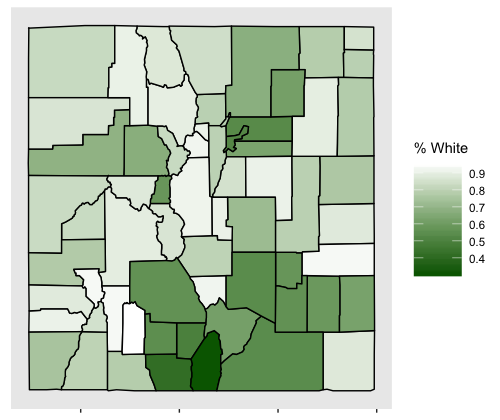
\includegraphics[width=0.4\linewidth]{/Users/tdounias/Desktop/Reed_Senior_Thesis/maps/pct_white_county_map} 
  
  }
  
  \caption[Map of Percentage of White Residents Per County]{Map of Percentage of White Residents Per County}\label{fig:white pct map}
  \end{figure}
  
  The State Capital is Denver. Colorado is split into 64 Counties, of
  which the most populous are, in no particular order, the following
  eight: El Paso, Denver, Arapahoe, Jefferson, Adams, Larimer, Boulder,
  and Douglas. These counties comprise 73\% of the total population of
  Colorado.
  
  \begin{longtable}[]{@{}lrrl@{}}
  \toprule
  County & Total Population & CO Population \% & Largest Metro
  Area\tabularnewline
  \midrule
  \endhead
  Adams & 441603 & 0.0878079 & Denver-Aurora-Lakewood Metro
  Area\tabularnewline
  Arapahoe & 572003 & 0.1137365 & Denver-Aurora-Lakewood Metro
  Area\tabularnewline
  Boulder & 294567 & 0.0585714 & Boulder\tabularnewline
  Denver & 600158 & 0.1193348 & Denver\tabularnewline
  Douglas & 285465 & 0.0567616 & Denver-Aurora-Lakewood Metro
  Area\tabularnewline
  El Paso & 622263 & 0.1237301 & Colorado Springs\tabularnewline
  Jefferson & 534543 & 0.1062880 & Denver-Aurora-Lakewood Metro
  Area\tabularnewline
  Larimer & 299630 & 0.0595781 & Fort COllins\tabularnewline
  Other & 1378964 & 0.2741917 &\tabularnewline
  Colorado & 5029196 & 100.0000000 &\tabularnewline
  \bottomrule
  \end{longtable}
  
  \subsection{Voting in Colorado}\label{voting-in-colorado}
  
  Each County individually administrates local, coordinated, primary, and
  general elections, under the supervision of the Colorado Secretary of
  State. This means that each county individually handles the voters
  registered in that county. Unsurprisingly, the same eight most populous
  counties are also the counties with the majority of registered voters,
  as their registrants comprise 73\% of total Colorado registered voters
  (as of November 2017). As Table shows, these eight counties have a
  registration rate between 60-80\%, compared to a Colorado-wide rate of
  about 67\%. Registration rates for all counties are also graphically
  depicted in Figure 2.
  
  \begin{longtable}[]{@{}lrlr@{}}
  \toprule
  \begin{minipage}[b]{0.10\columnwidth}\raggedright\strut
  County\strut
  \end{minipage} & \begin{minipage}[b]{0.23\columnwidth}\raggedleft\strut
  Total Registered Voters\strut
  \end{minipage} & \begin{minipage}[b]{0.30\columnwidth}\raggedright\strut
  County Voter Registration Rate\strut
  \end{minipage} & \begin{minipage}[b]{0.26\columnwidth}\raggedleft\strut
  \% of Statewide Registrants\strut
  \end{minipage}\tabularnewline
  \midrule
  \endhead
  \begin{minipage}[t]{0.10\columnwidth}\raggedright\strut
  Adams\strut
  \end{minipage} & \begin{minipage}[t]{0.23\columnwidth}\raggedleft\strut
  270303\strut
  \end{minipage} & \begin{minipage}[t]{0.30\columnwidth}\raggedright\strut
  0.612095026528352\strut
  \end{minipage} & \begin{minipage}[t]{0.26\columnwidth}\raggedleft\strut
  0.0723838\strut
  \end{minipage}\tabularnewline
  \begin{minipage}[t]{0.10\columnwidth}\raggedright\strut
  Arapahoe\strut
  \end{minipage} & \begin{minipage}[t]{0.23\columnwidth}\raggedleft\strut
  410546\strut
  \end{minipage} & \begin{minipage}[t]{0.30\columnwidth}\raggedright\strut
  0.717733997898612\strut
  \end{minipage} & \begin{minipage}[t]{0.26\columnwidth}\raggedleft\strut
  0.1099391\strut
  \end{minipage}\tabularnewline
  \begin{minipage}[t]{0.10\columnwidth}\raggedright\strut
  Boulder\strut
  \end{minipage} & \begin{minipage}[t]{0.23\columnwidth}\raggedleft\strut
  237091\strut
  \end{minipage} & \begin{minipage}[t]{0.30\columnwidth}\raggedright\strut
  0.804879704787026\strut
  \end{minipage} & \begin{minipage}[t]{0.26\columnwidth}\raggedleft\strut
  0.0634900\strut
  \end{minipage}\tabularnewline
  \begin{minipage}[t]{0.10\columnwidth}\raggedright\strut
  Denver\strut
  \end{minipage} & \begin{minipage}[t]{0.23\columnwidth}\raggedleft\strut
  450616\strut
  \end{minipage} & \begin{minipage}[t]{0.30\columnwidth}\raggedright\strut
  0.750828948376927\strut
  \end{minipage} & \begin{minipage}[t]{0.26\columnwidth}\raggedleft\strut
  0.1206694\strut
  \end{minipage}\tabularnewline
  \begin{minipage}[t]{0.10\columnwidth}\raggedright\strut
  Douglas\strut
  \end{minipage} & \begin{minipage}[t]{0.23\columnwidth}\raggedleft\strut
  237659\strut
  \end{minipage} & \begin{minipage}[t]{0.30\columnwidth}\raggedright\strut
  0.832532884942112\strut
  \end{minipage} & \begin{minipage}[t]{0.26\columnwidth}\raggedleft\strut
  0.0636421\strut
  \end{minipage}\tabularnewline
  \begin{minipage}[t]{0.10\columnwidth}\raggedright\strut
  El Paso\strut
  \end{minipage} & \begin{minipage}[t]{0.23\columnwidth}\raggedleft\strut
  445708\strut
  \end{minipage} & \begin{minipage}[t]{0.30\columnwidth}\raggedright\strut
  0.716269487338955\strut
  \end{minipage} & \begin{minipage}[t]{0.26\columnwidth}\raggedleft\strut
  0.1193551\strut
  \end{minipage}\tabularnewline
  \begin{minipage}[t]{0.10\columnwidth}\raggedright\strut
  Jefferson\strut
  \end{minipage} & \begin{minipage}[t]{0.23\columnwidth}\raggedleft\strut
  422362\strut
  \end{minipage} & \begin{minipage}[t]{0.30\columnwidth}\raggedright\strut
  0.790136621375642\strut
  \end{minipage} & \begin{minipage}[t]{0.26\columnwidth}\raggedleft\strut
  0.1131033\strut
  \end{minipage}\tabularnewline
  \begin{minipage}[t]{0.10\columnwidth}\raggedright\strut
  Larimer\strut
  \end{minipage} & \begin{minipage}[t]{0.23\columnwidth}\raggedleft\strut
  250626\strut
  \end{minipage} & \begin{minipage}[t]{0.30\columnwidth}\raggedright\strut
  0.836451623669192\strut
  \end{minipage} & \begin{minipage}[t]{0.26\columnwidth}\raggedleft\strut
  0.0671145\strut
  \end{minipage}\tabularnewline
  \begin{minipage}[t]{0.10\columnwidth}\raggedright\strut
  Other\strut
  \end{minipage} & \begin{minipage}[t]{0.23\columnwidth}\raggedleft\strut
  1009392\strut
  \end{minipage} & \begin{minipage}[t]{0.30\columnwidth}\raggedright\strut
  ---\strut
  \end{minipage} & \begin{minipage}[t]{0.26\columnwidth}\raggedleft\strut
  0.2703027\strut
  \end{minipage}\tabularnewline
  \begin{minipage}[t]{0.10\columnwidth}\raggedright\strut
  Colorado\strut
  \end{minipage} & \begin{minipage}[t]{0.23\columnwidth}\raggedleft\strut
  3734303\strut
  \end{minipage} & \begin{minipage}[t]{0.30\columnwidth}\raggedright\strut
  ---\strut
  \end{minipage} & \begin{minipage}[t]{0.26\columnwidth}\raggedleft\strut
  100.0000000\strut
  \end{minipage}\tabularnewline
  \bottomrule
  \end{longtable}
  
  \begin{figure}
  
  {\centering 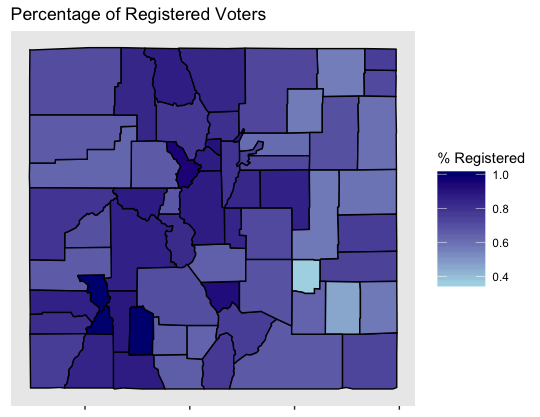
\includegraphics[width=0.4\linewidth]{/Users/tdounias/Desktop/Reed_Senior_Thesis/maps/pct_registered_county_map} 
  
  }
  
  \caption[Map of Registration Rates Per County]{Map of Registration Rates Per County}\label{fig:reg per county map}
  \end{figure}
  
  In terms of Party registration, Colorado as a whole leans democratic by
  a very narrow margin. This is also reflected in the state's Cook
  Partisan Voting Index of D +1, making it a solidly purple battleground
  state (Figure 3).
  
  \begin{figure}
  
  {\centering 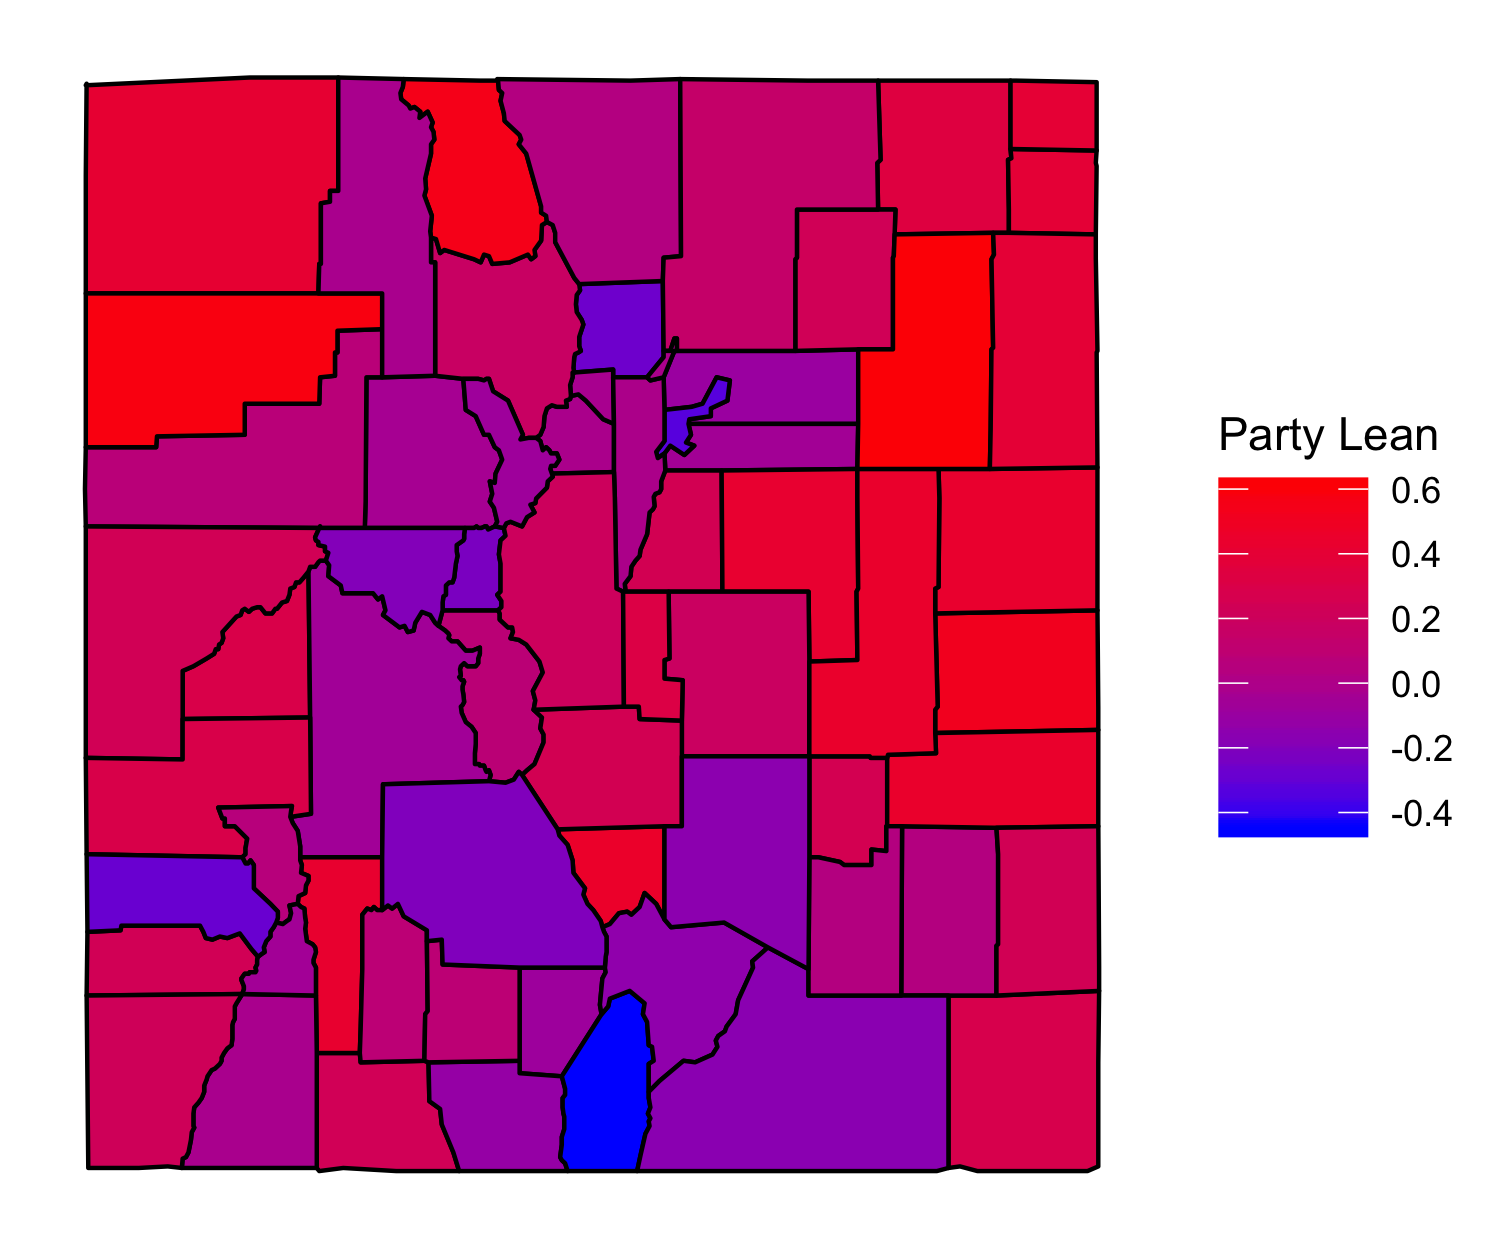
\includegraphics[width=0.4\linewidth]{/Users/tdounias/Desktop/Reed_Senior_Thesis/maps/party_affiliation_county_map} 
  
  }
  
  \caption[Map of Party Affiliation Per County]{Map of Party Affiliation Per County}\label{fig:party reg per county map}
  \end{figure}
  
  In the past 25 years, there have been a series of key changes in the way
  Colorado administers elections, in relation to Vote By Mail and other
  reforms targeted and expanding the democratic franchise. In 1992,
  Colorado introduced no-excuse absentee voting, allowing voters to either
  physically pick up a mail ballot at a Vote Center or County Office, or
  have a ballot mailed to them prior to election day. In 2008, this reform
  was expanded to a permanent Vote-By-Mail system, which gave voters the
  option to be permanently put on a list of addresses that received mail
  ballots prior to the election. The State also entered a transitional
  status to full mail elections, giving counties the option to make all
  coordinated local elections, general elections, and primary elections
  exclusively VBM. In 2013, the Colorado State Legislature passed
  HB13-1303: The Voter Access and Modernized Elections Act, which mandated
  that every voter currently registered receive a mail ballot for all
  future elections. The Act also expanded the use of Vote Centers instead
  of traditional polling places, instituted same-day voter registration,
  and revamped the way active and inactive voter status was designated on
  voter rolls--more on this in future sections. These changes are
  summarised in Table.
  
  \begin{longtable}[]{@{}ll@{}}
  \toprule
  \begin{minipage}[b]{0.04\columnwidth}\raggedright\strut
  Year\strut
  \end{minipage} & \begin{minipage}[b]{0.90\columnwidth}\raggedright\strut
  Key Changes\strut
  \end{minipage}\tabularnewline
  \midrule
  \endhead
  \begin{minipage}[t]{0.04\columnwidth}\raggedright\strut
  1992\strut
  \end{minipage} & \begin{minipage}[t]{0.90\columnwidth}\raggedright\strut
  No Excuse Absentee Statewide Implementation\strut
  \end{minipage}\tabularnewline
  \begin{minipage}[t]{0.04\columnwidth}\raggedright\strut
  2008\strut
  \end{minipage} & \begin{minipage}[t]{0.90\columnwidth}\raggedright\strut
  Permanent No-Excuse VBM Lists, Option of Full-VBM Elections\strut
  \end{minipage}\tabularnewline
  \begin{minipage}[t]{0.04\columnwidth}\raggedright\strut
  2013\strut
  \end{minipage} & \begin{minipage}[t]{0.90\columnwidth}\raggedright\strut
  Automatic Mail Ballot System Implemented Statewide, Established Vote
  Centers\strut
  \end{minipage}\tabularnewline
  \bottomrule
  \end{longtable}
  
  Colorado presents such an interesting case for research on Vote By Mail
  exactly because it has gone through such a long transitional process to
  reach its current elections system. It has steadily developed voting
  policy through a mixture of state mandates, county action, and outside
  policy motivations. It gives researchers access to approximatelly 22
  years during which at least part of the state conducted elections
  partially by mail, making comparative, county- or individual- level case
  studies particularly alluring.
  
  \section{Getting the Data}\label{getting-the-data}
  
  This thesis relies on county and individual level models to draw
  conclusions on voting behaviours, and how they are affected by voting
  method. As such, the data I need will optimally contain the following:
  
  \begin{itemize}
  \item
    \textbf{County and individual level demographic characteristics}:
    race, gender, urban population
  \item
    \textbf{County and individual level voting data}: turnout, party
    registration, total registrants
  \item
    \textbf{Information on individual elections}: date, ballots cast,
    voting methods, county, election descriptions
  \end{itemize}
  
  In the process of my research, I have acquired sufficient data to cover
  the second and third of these areas. I was unable to procure individual
  level data on demographic characteristics apart from gender, age, and
  party registration. However, reasonable conclusions can still be drawn
  from county or precinct aggregates.
  
  \subsection{Sources and first glance}\label{sources-and-first-glance}
  
  I used two sources of data: Colorado voter records procured from the
  Colorado Secretary of State's office, and demographic data from the 2010
  US Census. In the process of procuring these data I was aided by a
  series of other researchers and professionals with experience in the
  field of elections administration; they are mentioned in my
  acknowledgements.
  
  \subsubsection{2010 US Census}\label{us-census}
  
  The US Census is conducted country-wode every ten years, with the goal
  of procuring accurate data on the demographic characteristics of the
  population. The Census uses a combination of federal field workers
  conducting door-to-door canvassing and statistical methods for data
  aggregation. From the 2010 Census--which is publically available
  online--I get total population counts, characteristics on race, and
  rural/urban population counts for Colorado.
  
  I use two datasets from the Census. For both, the unit of observation is
  one of the 64 counties of Colorado, and both include the same total
  population counts. One contains racial demographic characteristics and
  the other contain percentages of rural and urban populations in each
  county. The racial demographic dataset needed some wrangling work to
  extract a percentage of white residents in each county. Individuals were
  coded as ``white'' when they identified as exclusivelly white--this
  doesn't include mixed-race individuals reporting white ancestry.
  
  \subsubsection{Colorado Voter Files}\label{colorado-voter-files}
  
  As any state, Colorado maintains a statewide registry of all currently
  registered voters. This registry is typically under the purview of the
  Secretary of State--in this case, Wayne W. Williams. Voter Registration
  Files are constantly updated with new information on existing voters,
  new voters, or with the removal of inactive or otherwise ineligible
  voters. Therefore, this file will be different every time it is accessed
  or shared. Based on when this file is accessed, only a ``snapshot'' of
  the file can be obtained. I have managed to procure ``snapshots'' for
  each year between 2012 and 2017.
  
  Similarly with VRFs, a Voter History File is maintained and constantly
  updated by the state. This file is uniquelly connected to its VRF: only
  voters showing up as registrants will have their histories included. I
  have similarly procured ``snapshots'' of the Voter History File for the
  years between 2012 and 2017.
  
  In the Voter Registration files, the unit of observation is the
  individual voter, and all variables are initially coded as character
  strings. Each voter is assigned a unique voter ID, which serves as a
  point of refference between the two files. Broadly speaking, data in
  this file can be divided between three categories: first, personal
  identification information like address, ZIP code, or phone number;
  second, demographic information like age and gender; third, information
  pertinent to elections administration like congressional district, local
  elections for which the individual should receive a ballot, voter ID,
  and party registration. I will further elaborate on relevant variables
  in the wrangling section.
  
  In the Voter History files, the unit of observation here is a single
  ballot cast, and all variables are initially coded as character strings.
  This means that for each voter registered--and so included in the
  VRF--the history file should contain an observation for each time they
  voted. This file includes two types of data: first, identifiers for the
  election like county, date, description, and type; second, identifiers
  for the individual vote including voter ID and voting method.
  
  \section{Wrangling the Data}\label{wrangling-the-data}
  
  The process of ``wrangling'' refers to manipulating the data into a form
  that can then be used fo graphing, exploratory data analysis, modelling,
  or presentation. In this case, wrangling also included aggregating data
  across multiple sources and datasets. For this purpose, I made heavy use
  of the tidyverse R package, and in particular the dplyr package. In this
  section I will go through some of the key problems encountered during
  the wrangling of these data, and then discuss the final form each
  variable takes.
  
  \subsection{Initial Problems with the 2017 Voter File and
  Solution}\label{initial-problems-with-the-2017-voter-file-and-solution}
  
  The first major issue I encountered--which merits discussion in its own
  section--derives from the aforementioned fact that the voter records I
  had access to are ``snapshots''. What this means, is that for each
  person in each year of voter registration files, I will have their
  corresponding history files for all ballots they have cast in Colorado,
  but not their own history of registration and migration. If, say, a
  voter moved from Boulder County to Summit County, I would have their
  votes in Boulder County show up in the voter history file, but them
  being registered in Summit. If you recall the turnout calculations
  specified earlier on, this implies an overestimation when looking back
  at elections that happened some time before the date of the
  ``snapshot''. Additionally, ``snapshots'' of current voter files do not
  reflect voters dropping off the rolls for whatever reason--death, moving
  out of the state, long term inactivity, non-confirmable personal data
  etc. Since for these voters the history files would also not be
  included, the issue created is less one of overestimation of turnout
  like before, but just the inclusion of additional room for error that is
  created when subtracting one from the denominator and enumerator of
  turnout.
  
  This was a significant problem from the beginning of this thesis, since
  I started out with only one ``snapshot'' from 2017. After going through
  turnout calculations, a significant majority of counties appeared to
  have turnout exceeding 100\%, particularly for years between 2000 and
  2012. This was, to put it mildly, concerning. With the help of my
  advisers, I was able to procure similar ``snapshots'' for each year
  between 2012-2016. After similar calculations, I returned the following
  graph for the eight most populous counties as described above, including
  different shapes for election type, colors for county, and a vertical
  line at 2013 to signify the latest major change in how Colorado
  administers elections:
  
  \begin{figure}
  
  {\centering 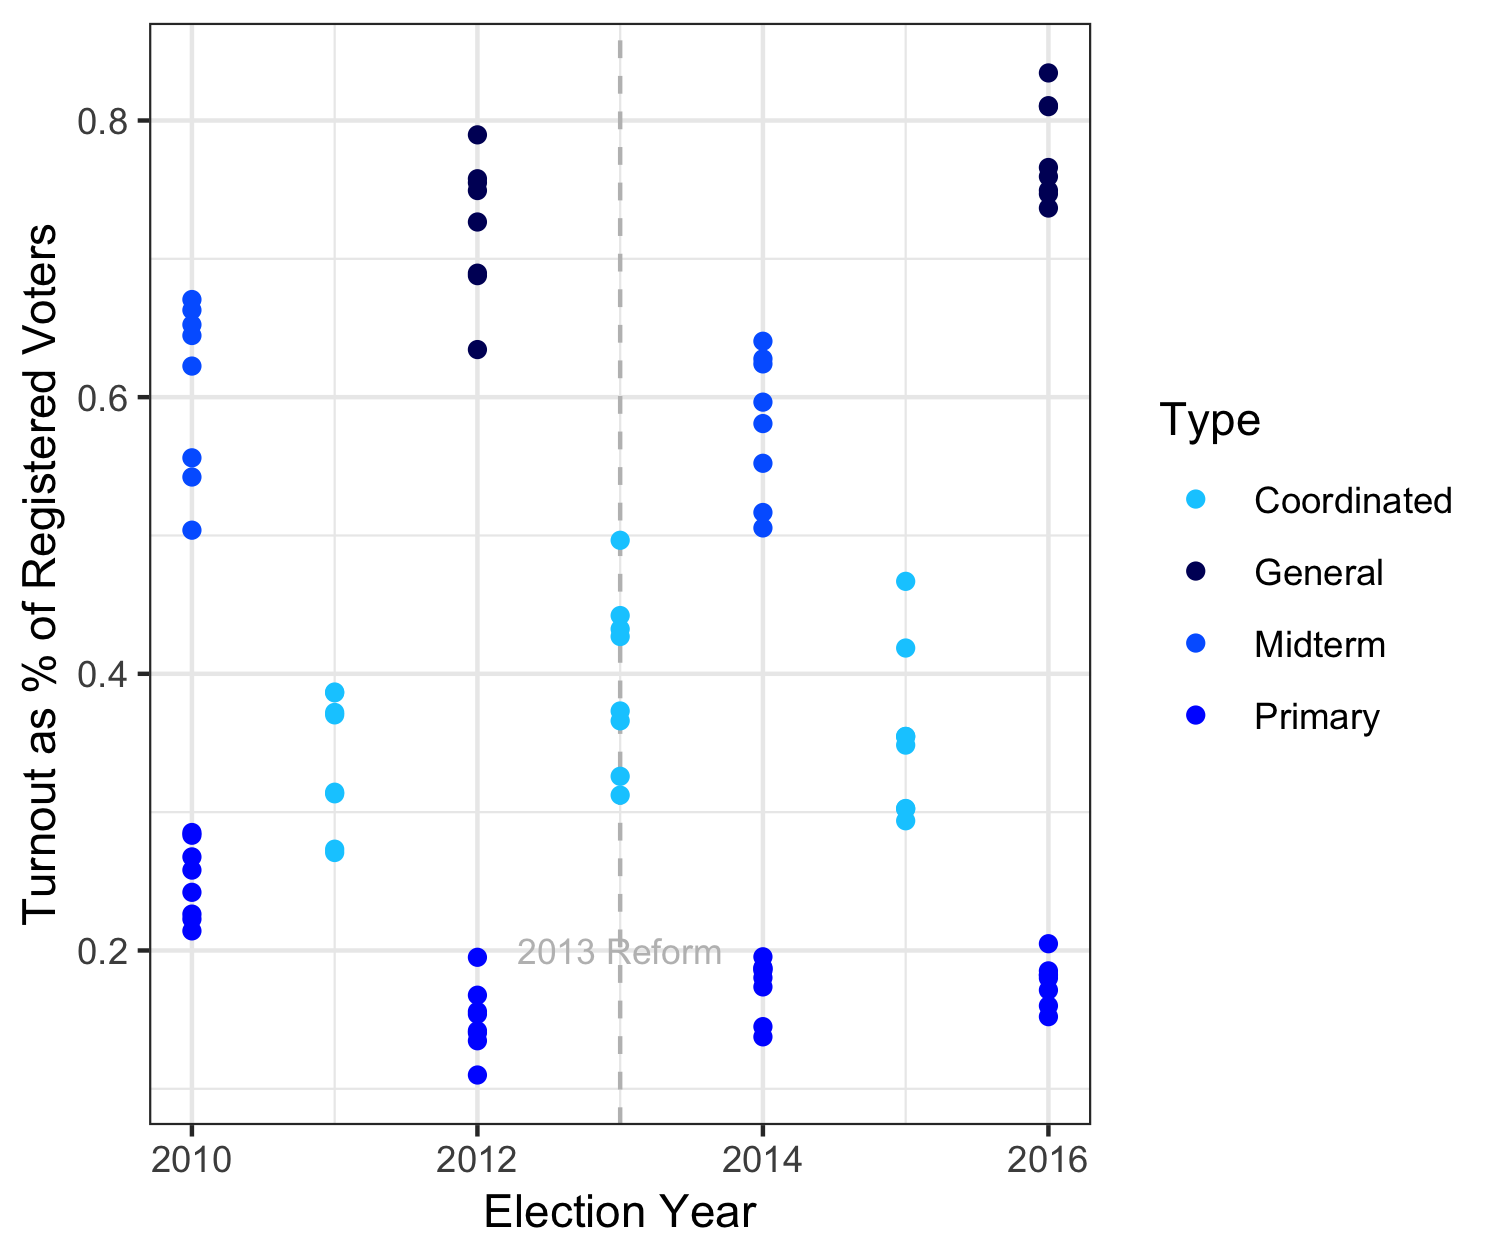
\includegraphics[width=0.4\linewidth]{/Users/tdounias/Desktop/Reed_Senior_Thesis/plots/colorado_bigeight_turnout_graph} 
  
  }
  
  \caption[Turnout Plot for Eight Largest Colorado Counties, 2012-2016]{Turnout Plot for Eight Largest Colorado Counties, 2012-2016}\label{fig:big eight turnout plot}
  \end{figure}
  
  To also further illustrate the in-county migration and dropped voter
  problem, I created a graph that includes logged total counts of
  registered voters calculated using the 2017 and the 2012-2016 files. The
  plot also includes a line at y=x. If in-Colorado migration and dropped
  voters are not an issue, most points on this graph should be at this
  line.
  
  \begin{figure}
  
  {\centering 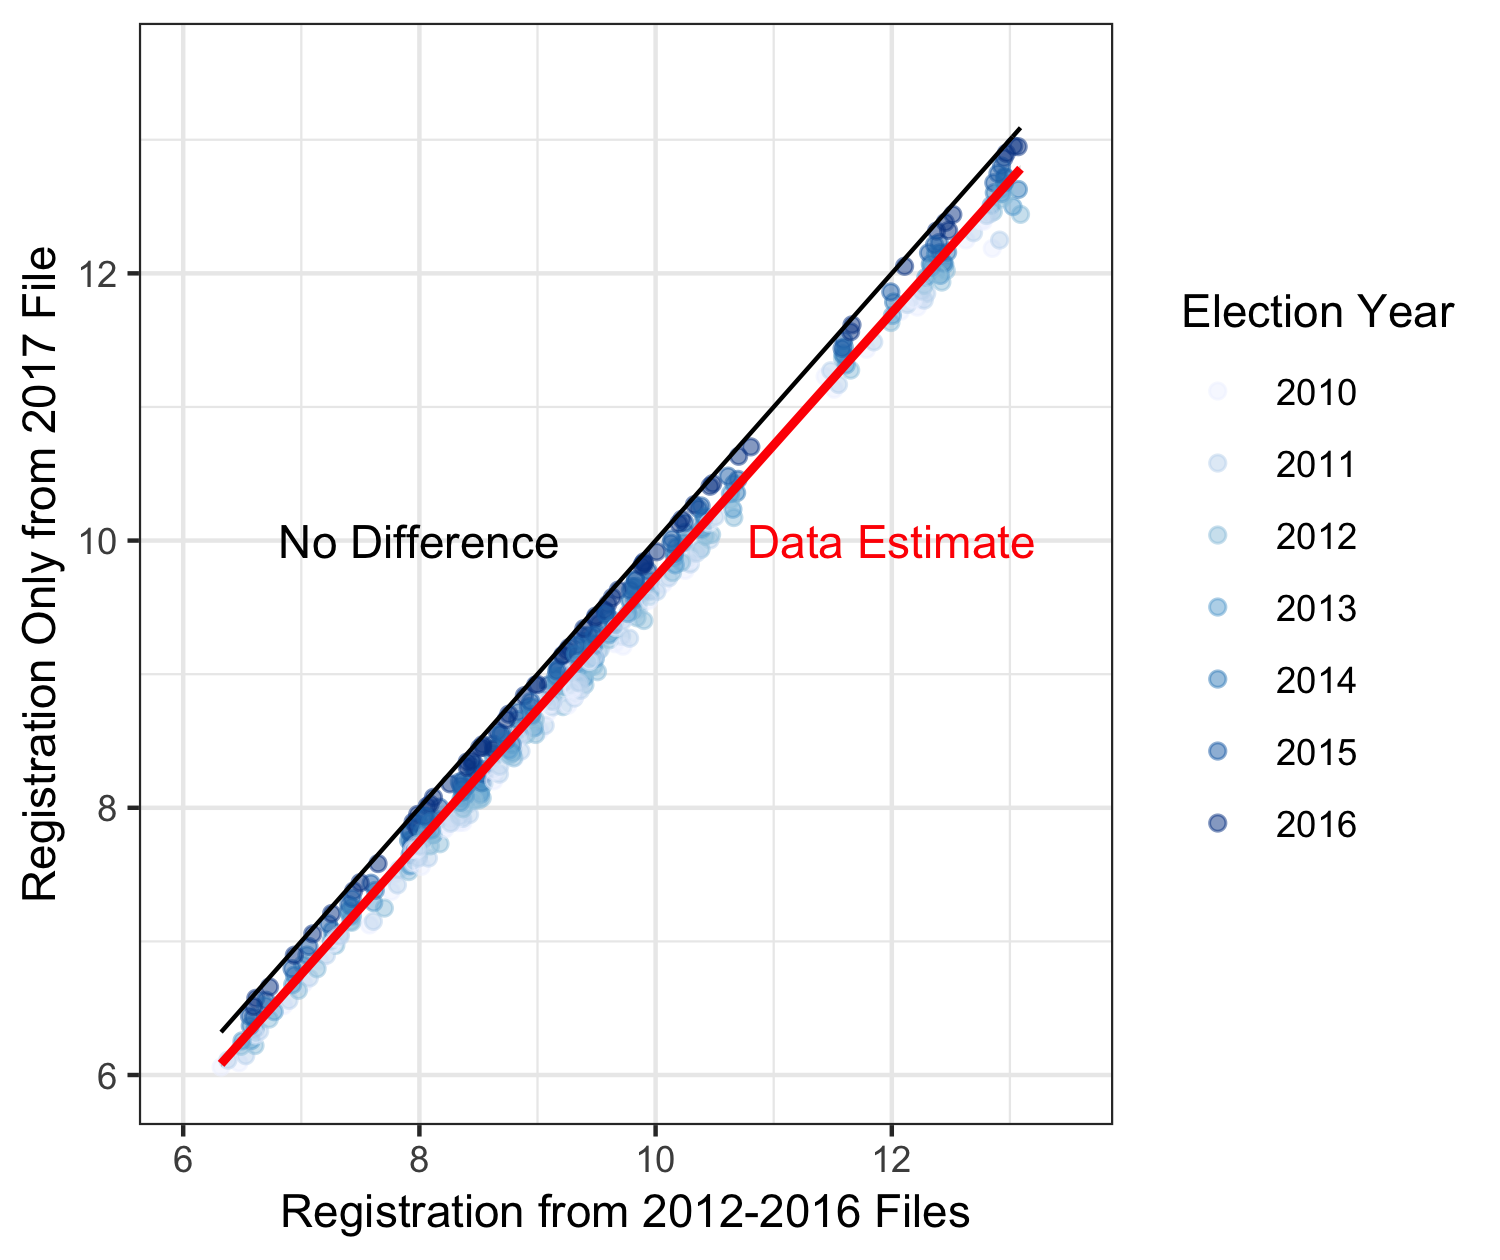
\includegraphics[width=0.4\linewidth]{/Users/tdounias/Desktop/Reed_Senior_Thesis/plots/county_migration_A} 
  
  }
  
  \caption[Comparison of registration count methods]{Comparison of registration count methods}\label{fig:county migration A}
  \end{figure}
  
  Two things should be clear from this plot. First, there is significant
  deviation between the counts using just the 2017 file and all files
  across years. Specifically, the 2017 count consistently underestimates
  the total amount of registered voters--this is shown by the red linear
  model smoothing line. This consistent difference confirms the hypothesis
  that there is a substantial benefit to using ``snapshots'' for multiple
  years. Second, counts get more accurate the closer to 2017 we get. This
  should be even more apparent in the following graph, which limits the
  scale to only some high registration counties, and adds a shape
  indicator for county:
  
  \begin{figure}
  
  {\centering 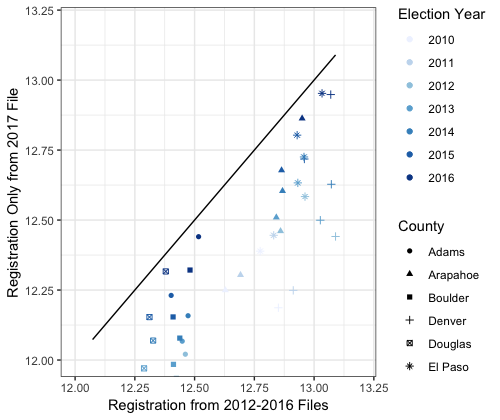
\includegraphics[width=0.4\linewidth]{/Users/tdounias/Desktop/Reed_Senior_Thesis/plots/county_migration_B} 
  
  }
  
  \caption[Comparison of registration count methods only for a few counties, 2012-2016]{Comparison of registration count methods only for a few counties, 2012-2016}\label{fig:county migration B}
  \end{figure}
  
  Here the structure of the data becomes clear: for each county, there are
  a series of almost vertically distributed points, which get closer to
  the y = x line the closer the counts get to 2017. Through this series of
  tests, it became clear that using multiple years of data was necessary
  in order to conduct an accurate test of my hypotheses. My selection was
  later vindicated, when looking at comparisons between reported rates of
  turnout\footnote{Turnout is calculated over all registered voters} and
  turnout calculated through my dataset for the 2014 midterm election:
  
  \begin{figure}
  
  {\centering 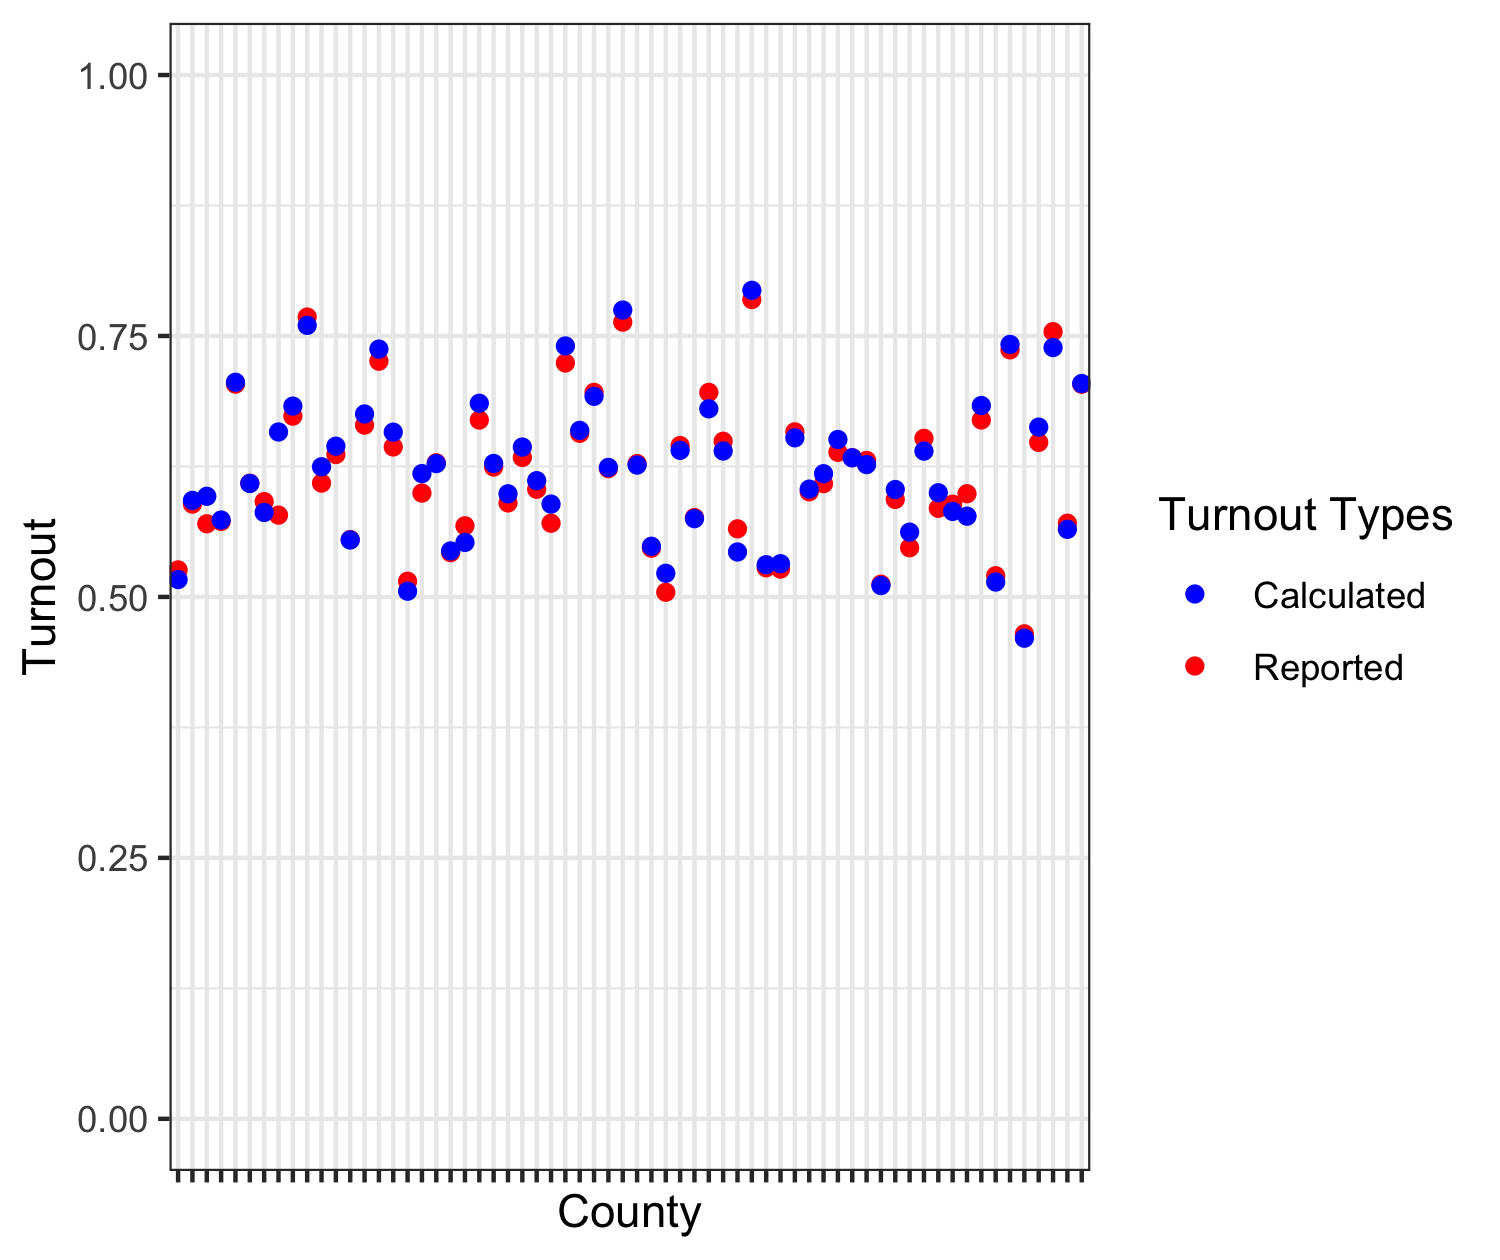
\includegraphics[width=0.4\linewidth]{/Users/tdounias/Desktop/Reed_Senior_Thesis/plots/Calc_vs_rep_turnout} 
  
  }
  
  \caption[Comparison of reported and calculated turnout for 2014 midterms across county]{Comparison of reported and calculated turnout for 2014 midterms across county}\label{fig:comp turnout 2014}
  \end{figure}
  
  The differences are insignificant. They exist because of ``noise'' added
  on because of errors in the data, misreporting, private voter
  registration files, voters dropped before the ``snapshot'' occured, and
  other similar factors.
  
  \subsection{Other Wrangling Issues
  Faced}\label{other-wrangling-issues-faced}
  
  Suffice to say, wrangling data was the majority of the work that went
  into this thesis. Doing a full account would probably read like the
  world's most cliche crime novel: a series of elusive final datasets, a
  plucky yet occassionally naive young detective, two wisened mentors,
  clues, dead ends, frustration, compromise, and\ldots{}spreadsheets. I
  will spare the reader the whole story, but I will include a
  non-comprehensive list of some of the difficulties associated with
  wrangling voter files, as it was a crucial part of the learning process
  I underwent while doing my research.
  
  \textbf{Missing Values}: The decision on how to deal with missing
  values--or NAs--in a dataset is a lot more important than it may
  initially seem. A first, intuitive reaction might be to just disregard
  them; however this works under the assumption that there is no structure
  inherent to why these data are missing! To give just two examples, in
  the data I have collected, the PARTY value for the 2015 voter
  registration file is missing. If I excluded all observations with
  missing PARTY values, I would be excluding a fifth of my data. Missing
  values were also present in the VOTING\_METHOD variable of the voter
  history files. While this may have seemed troubling, after closer
  examination it was revealed that the vast majority of such missing
  values was concentrated in Jefferson County, and in elections prior to
  2002. Therefore, these observations could be ignored, since they played
  no role in my final dataset. The conclusion should be that choices made
  on exclusion, inclusion, or estimation of missing data are very
  important, and should be taken with much care and consideration for the
  underlying structure of the data.
  
  \textbf{Data Input Errors}: Is ``Greece'' a legitimate voting method?
  Probably not. However, ``Greece'' did show up as a value in the
  VOTING\_METHOD variable for my 2012 voter history file snapshot. This
  may have occured for a series of reasons, like data reading issues--the
  data I acquired had changed hands some times, and also changed platforms
  between STATA and R--or issues at time of input--each county counts
  votes individually, and \emph{then} the state aggregates the data--, or
  some bug in my code. Having adequately checked for the later of these
  reasons, I treated all values that seemed more likelly than not to be
  errors as NAs. There were not many of these--less than .001\% of my
  data--but they were a hassle to find, analyze, and then recode into some
  useful value.
  
  \textbf{Data Size}: Nothing to write home about here, just an
  observation that multiple voter registration files can be \emph{huge},
  which puts considerable strain on a computer's processing power. This
  means that wrangling has to comprise of a series of careful, deliberate
  moves. Brute force should be discouraged, as a dead end means several
  hours of melodic computer fan panic.
  
  \textbf{Joining, Merging, Spreading, and the Multiplicity of Levels}:
  For the data to end up in any functional shape, it eventually becomes
  necessary to start joining datasets. Thankfully, a clear division of
  modelling tasks between county and individual level models means that
  joining on COUNTY or VOTER\_ID is ideal, and fairly straightforward. As
  will become clear in later sections, I also had to consider the variety
  of different units of observation, specifically: county, individual,
  ballot, election, county-by-election.
  
  \subsection{Final Variable
  Specifications}\label{final-variable-specifications}
  
  After the conclusion of the wrangling process, the resulting dataset
  included a series of discrete and continuous variables. I will briefly
  outline them here, along with their range and values.
  
  \begin{itemize}
  \tightlist
  \item
    VOTER\_ID: Discrete variable, unique value given to each individual
    voter. Useful for merging.
  \item
    COUNTY: Discrete variable, the 64 counties of Colorado.
  \item
    REGISTRATION\_DATE: Discrete variable, date of registration for each
    registrant. Useful to get total registrants on election day.
  \item
    TURNOUT: Continuous variable, in the range {[}0,1{]}. The response
    variable for my county-level models.
  \item
    ELECTION\_TYPE: Discrete variable, the four types of elections:
    Primary, Coordinated, Midterm, Presidential.
  \item
    ELECTION\_DATE: Discrete variable, self-explanatory.
  \item
    VBM\_PCT: Continuous variable, in the range {[}0,1{]}. This is the
    focus of my analysis, as it counts the percentage of total ballots
    that were mail ballots.
  \item
    PCT\_WHITE: Continuous variable, in the range {[}0,1{]}. Percentage of
    white residents per county.
  \item
    PCT\_URBAN: Continuous variable, in the range {[}0,1{]}. Percentage of
    urban residents per county.
  \item
    PARTY: Discrete variable. For each voter, the party they are
    registered with. Can be: Republican, Democrat, Other, or Unaffiliated.
  \item
    GENDER: Discrete binary variable, Male or Female.
  \item
    AGE: The age of the individual registrant.
  \item
    VOTING\_METHOD: The method used by an individual voter to cast their
    ballot. Is coded as either VBM or In Person, according to the
    following table:
  \end{itemize}
  
  \begin{longtable}[]{@{}lll@{}}
  \toprule
  \begin{minipage}[b]{0.13\columnwidth}\raggedright\strut
  Voting Method\strut
  \end{minipage} & \begin{minipage}[b]{0.63\columnwidth}\raggedright\strut
  Description of Method\strut
  \end{minipage} & \begin{minipage}[b]{0.15\columnwidth}\raggedright\strut
  Final Designation\strut
  \end{minipage}\tabularnewline
  \midrule
  \endhead
  \begin{minipage}[t]{0.13\columnwidth}\raggedright\strut
  Absentee Carry\strut
  \end{minipage} & \begin{minipage}[t]{0.63\columnwidth}\raggedright\strut
  Voters who carried an absentee ballot with them from an early voting
  location\strut
  \end{minipage} & \begin{minipage}[t]{0.15\columnwidth}\raggedright\strut
  VBM\strut
  \end{minipage}\tabularnewline
  \begin{minipage}[t]{0.13\columnwidth}\raggedright\strut
  Absentee Mail\strut
  \end{minipage} & \begin{minipage}[t]{0.63\columnwidth}\raggedright\strut
  Voters who were sent an absentee ballot, and mailed it in\strut
  \end{minipage} & \begin{minipage}[t]{0.15\columnwidth}\raggedright\strut
  VBM\strut
  \end{minipage}\tabularnewline
  \begin{minipage}[t]{0.13\columnwidth}\raggedright\strut
  Early Voting\strut
  \end{minipage} & \begin{minipage}[t]{0.63\columnwidth}\raggedright\strut
  Voters who physically went to an Early Voting location and voted\strut
  \end{minipage} & \begin{minipage}[t]{0.15\columnwidth}\raggedright\strut
  In Person\strut
  \end{minipage}\tabularnewline
  \begin{minipage}[t]{0.13\columnwidth}\raggedright\strut
  In Person\strut
  \end{minipage} & \begin{minipage}[t]{0.63\columnwidth}\raggedright\strut
  Voters who physically went to a polling place and voted on paper\strut
  \end{minipage} & \begin{minipage}[t]{0.15\columnwidth}\raggedright\strut
  In Person\strut
  \end{minipage}\tabularnewline
  \begin{minipage}[t]{0.13\columnwidth}\raggedright\strut
  Mail Ballot\strut
  \end{minipage} & \begin{minipage}[t]{0.63\columnwidth}\raggedright\strut
  Vote By Mail\strut
  \end{minipage} & \begin{minipage}[t]{0.15\columnwidth}\raggedright\strut
  VBM\strut
  \end{minipage}\tabularnewline
  \begin{minipage}[t]{0.13\columnwidth}\raggedright\strut
  Polling Place\strut
  \end{minipage} & \begin{minipage}[t]{0.63\columnwidth}\raggedright\strut
  Traditional polling place voting, discontinued in 2013\strut
  \end{minipage} & \begin{minipage}[t]{0.15\columnwidth}\raggedright\strut
  In Person\strut
  \end{minipage}\tabularnewline
  \begin{minipage}[t]{0.13\columnwidth}\raggedright\strut
  Vote Center\strut
  \end{minipage} & \begin{minipage}[t]{0.63\columnwidth}\raggedright\strut
  Voters who cast their ballots at Vote Centers\strut
  \end{minipage} & \begin{minipage}[t]{0.15\columnwidth}\raggedright\strut
  In Person\strut
  \end{minipage}\tabularnewline
  \bottomrule
  \end{longtable}
  
  \section{Model Parametrization}\label{model-parametrization}
  
  \subsection{Notation for predictors}\label{notation-for-predictors}
  
  There are four distinct types of predictors for use in these models.
  
  \subsubsection{County and County-per-Election
  Level}\label{county-and-county-per-election-level}
  
  First, I define the following indicator variables:
  
  \(\bullet ~x_c,~for~c\in [1, 64]\), dummy variables for each county in
  Colorado.
  
  Furthermore, I have two county-level predictors:
  
  \(\bullet~x^{white~\%}\), a vector of length 64, percentage of county
  population that identifies as only white.
  
  \(\bullet~x^{urban~\%}\), a vector of length 64, percentage of county
  population living in an urban area.
  
  There are two other predictors, varying by county and election. These
  are of particular interest, as one is the response variable for my
  county-level models, and the other is the variable of interest for this
  study. Specifically:
  
  \(\bullet~x^{mail~vote~\%}\), a vector of percentage of votes that was
  cast using mail ballots, per county and election.
  
  \(\bullet~y^{turnout~\%}\), a vector with turnout counts per county and
  election. Coded with a \(y\) to identify as a response variable
  
  Since the unit of observation for the county level models I will apply
  are all counties per election, I define an aggregate matrix of length
  equal to the number of elections times 64--the number of counties---,
  and width equal to 3. This matrix includes all county level predictors:
  \(X =(x^{white~\%},x^{urban~\%},x^{mail~vote~\%})\). Note that this
  matrix includes percentage of mail ballots cast, which is the variable
  whose coefficient I am interested in testing.
  
  \subsubsection{Election Level}\label{election-level}
  
  There are two exclusivelly election-level dicrete variables: year, and
  type of election. For both I define a series of indicator variables:
  
  \(\bullet ~w^{election~type}\), for each election type (Midterm, Primary
  , Coordinated, General).
  
  \(\bullet ~w^{election~year}\), for each election year, between 2010 and
  2016.
  
  I will also use \(year\) as a variable for models using smoothing
  splines. All election level predictors will be summarized for the
  purposes of modelling in the 9 by 2 matrix
  \(W = (w^{election~type}, w^{election~year})\).
  
  \subsubsection{Individual and Individual-per-Election
  Level}\label{individual-and-individual-per-election-level}
  
  The two aforementioned predictors--urban population and race--could be
  defined as aggregates of individual level observations. I also have five
  other distinct individual level variables:
  
  \(\bullet~z^{gender}\), a vector of discrete gender identifications for
  each voter, varying only by voter.
  
  \(\bullet~z^{age}\), a vector of age for each vote, varying by voter and
  election.
  
  \(\bullet~z^{party}\), a vector of party registration for each voter,
  varying by voter and election. Coded as Republican, Democratic, Other,
  or Unaffiliated.
  
  \(\bullet~z^{voted}\), with \(z^{voted}_{i,j} = 1\) if person i voted in
  election j, and \(z^{voted}_{i,j} = 0\) if they did not.
  
  \(\bullet~z^{mail~ballot}\), a vector of binary values depending on
  whether voting method was by mail for each voter, varying by voter and
  election. Coded 0 if the individual did not vote.
  
  Since the unit of observation for the individual level models I will
  apply are all individuals in a particular election, I define an
  aggregate matrix of length equal to the total number of voters, and
  width equal to 4. This matrix includes all individual level predictors:
  \(Z =(z^{gender}, z^{age}, z^{party}, z^{mail~ballot})\). The fourth
  variable defined in this section is the response variable in the
  individual level model, and as such is not included in the predictors.
  
  \subsection{County Level Models}\label{county-level-models}
  
  \textbf{Model 1} is a fixed-effects, bare-bones model that exclusivelly
  includes percentage of VBM votes, and dummy variables for year, election
  type, and county. Its call would look a bit like:
  
  \[y^{turnout~\%}_{c, l} \sim x^{mail~vote~\%}_{c, l}\beta_1 + \sum_{k = 1}^{4}w_{k, l}^{election~type}\beta_{k+1} + \sum_{j = 1}^{7}w_{j, l}^{election~year}\beta_{j+5} + \sum_{c = 1}^{64} x_c\beta_{c+13} \]
  
  Where k sums over the four types of election, j sums over years between
  2010 and 2016, c sums over counties, and l sums over elections
  
  \textbf{Model 2} A more informed baseline, model 1 plus variables of
  urban and white population:
  
  \[y^{turnout~\%}_{c, l} \sim x^{mail~vote~\%}_{c, el}\beta_1 + \sum_{k = 1}^{4}w_{k, l}^{election~type}\beta_{k+1} + \sum_{j = 1}^{7}w_{j, l}^{election~year}\beta_{j+5} + \]
  \[\sum_{c = 1}^{64} x_c\beta_{c+13} + x^{white~\%}_{c}\beta_{78} + x^{urban~\%}_{c}\beta_{79}\]
  This would be the ``individual'' level model from Gelman and Hill. I'm
  unsure what the ``group'' level for county would be. Maybe that part of
  the book would be more helpful for discerning effects on people's
  individual p-vote?
  
  Maybe more informative is what I did with exercise 12.2. The model tries
  to predict the concentration of a particular chemical based on treatment
  of children across time. Therefore the two levels are a visit by one
  individual child (here an election! so type, vbm\_pct, year) and
  predictors for that individual child that are stable across time, like
  treatment type, or demographics (here race and urban pop per county).
  
  This means I can fit a model only based on election facts, with a
  variable for county (models 1,3) or one that takes into account stable
  characteristics of the county (models 2, 4).
  
  \textbf{Model 3} A mixed-effects version of model 1, just adds mixed
  effects for county:
  
  \[y^{turnout~\%}_{c, l} \sim x^{mail~vote~\%}_{c, l}\beta_1 + \sum_{k = 1}^{4}w_{k, l}^{election~type}\beta_{k+1} + \sum_{j = 1}^{7}w_{j, l}^{election~year}\beta_{j+5} + \alpha_{[c],l}\]
  
  \[\alpha_{[c],l} \sim N(0, \sigma_{\alpha}^2)\]
  
  \textbf{Model 4} A mixed-effects version of model 2:
  
  \[y^{turnout~\%}_{c, l} \sim x^{mail~vote~\%}_{c, l}\beta_1 + \sum_{k = 1}^{4}w_{k, l}^{election~type}\beta_{k+1} + \sum_{j = 1}^{7}w_{j, l}^{election~year}\beta_{j+5} + \alpha_{[c],l}\]
  
  \[\alpha_{[c]l} \sim N(x^{white~\%}\gamma_{1} + x^{urban~\%}\gamma_{2}, \sigma_{\alpha}^2),~for~c = 1,...,64\]
  
  Where D is a 2 x 64 matrix of the county level predictors and \(\gamma\)
  a vector of coefficients for the county-level regression.
  
  \textbf{Model 5} During one of my discussions with Andrew, we discussed
  the possibility of making a model that answers the question: ``Does VBM
  affect counties with some particular characteristic \emph{for which I
  don't have data} more than others?'' As such, this model would
  substitute county-level effects with a set of 3-4 dummy variables
  created through my intuitive understanding of Colorado politics and
  counties. For example, maybe a distinciton between central Colorado
  urban counties, East Colorado plains counties, and West Colorado
  mountain counties. The model would look a bit like:
  
  \[y^{turnout~\%}_{c, l} \sim x^{mail~vote~\%}_{c, l}\beta_1 + \sum_{k = 1}^{4}w_{k, l}^{election~type}\beta_{k+1} + \]
  \[\sum_{j = 1}^{7}w_{j, l}^{election~year}\beta_{j+5} + \sum_{c = 1}^{n} x^{county~classification}_c\beta_{c+13}\]
  Where \(x^{county~classification}_c\) are \(n\) dummy variables, one for
  each county classification group.
  
  \textbf{Model 6} As a check on the previous model, run a Principle
  Components Analysis on full demographic data from the 2010 census, to
  classify counties in the same number of groups. This model would be
  expected to \emph{massively overfit}. Learning experience for all!
  
  \textbf{Note} All models can work as General Additive Models with some
  sort of non-linear smoothing function for year. Just replace
  \(\sum_{j = 1}^{7}w_j^{election~year}\beta_{j+5}\) with \(ns(year)\).
  
  \textbf{Model 7} In order to test the hypothesis that voting by mail
  varies by election type, I can also construct the following model, based
  on model 4:
  
  \[x^{mail~vote~\%}_{c, l} \sim \sum_{k = 1}^{4}w_{k, l}^{election~type}\beta_{k} + \sum_{j = 1}^{7}w_{j, l}^{election~year}\beta_{j+4} + \alpha_{[c]}\]
  \[\alpha_{[c],l} \sim N(x^{white~\%}\gamma_{1} + x^{urban~\%}\gamma_{2}, \sigma_{\alpha}^2),~for~c = 1,...,64\]
  This would predict whether there are specific county or election
  characteristics that increase the amount of mail ballots individuals
  cast.
  
  \subsection{Individual Level Models}\label{individual-level-models}
  
  This section follows directly from the intro to Gelman \& Hill's 11th
  chapter.
  
  \textbf{Model 8} As a baseline for all further analysis, a logistic
  regression that treats each vote in a single election as uniform across
  counties, as such not including any group-level predictors.
  
  \[P(z^{voted}_{i, l} = 1) = logit^{-1}(Z_{i, l}\delta + W_l\beta)\]
  
  Where matrices Z, Y are as described above, i is an indice for each
  voter, and l for each election. \(\delta, \beta\) are vectors of
  coefficients to be estimated.
  
  \textbf{Model 9} Add group level mixed effects and predictors.
  
  \[P(z^{voted}_{i, l} = 1) = logit^{-1}(Z_{i, l}\alpha + W_l\beta + \alpha_{[c],l})\]
  
  \[\alpha_{[c],l} \sim N(X_c \gamma, \sigma_{\alpha}^2),~for~c = 1,...,64\]
  
  Where \(X_c\) as defined above, and \(\gamma\) a vector of coefficients.
  
  \textbf{Model 10} Include extra model with EM algorithm applied to 2015
  data maybe?
  
  \chapter{Results}\label{results}
  
  \section{EDA}\label{eda}
  
  \section{Models}\label{models}
  
  \subsection{County Level Models}\label{county-level-models-1}
  
  \subsection{Individual Level Models}\label{individual-level-models-1}
  
  \chapter{Expanding on the Previous
  Models}\label{expanding-on-the-previous-models}
  
  \chapter*{Conclusion}\label{conclusion}
  \addcontentsline{toc}{chapter}{Conclusion}
  
  \setcounter{chapter}{4} \setcounter{section}{0}
  
  \appendix
  
  \backmatter
  
  \chapter{References}\label{references}
  
  \noindent
  
  \setlength{\parindent}{-0.20in} \setlength{\leftskip}{0.20in}
  \setlength{\parskip}{8pt}
  
  \hypertarget{refs}{}
  \hypertarget{ref-aldrich_rational_1993}{}
  Aldrich, J. H. (1993). Rational Choice and Turnout. \emph{American
  Journal of Political Science}, \emph{37}(1), 246--278.
  \url{http://doi.org/10.2307/2111531}
  
  \hypertarget{ref-ansolabehere_quality_2010}{}
  Ansolabehere, S., \& Hersh, E. (2010). The Quality of Voter Registration
  Records: A State-by-State Analysis. \emph{Institute for Quantitative
  Social Science and Caltech/MIT Voting Technology Project Working Paper}.
  Retrieved from
  \url{https://dataverse.harvard.edu/dataset.xhtml?persistentId=hdl:1902.1/18550}
  
  \hypertarget{ref-ansolabehere_validation:_2012}{}
  Ansolabehere, S., \& Hersh, E. (2012). Validation: What Big Data Reveal
  About Survey Misreporting and the Real Electorate. \emph{Political
  Analysis}, \emph{20}(04), 437--459.
  \url{http://doi.org/10.1093/pan/mps023}
  
  \hypertarget{ref-ansolabehere_adgn:_2017}{}
  Ansolabehere, S., \& Hersh, E. D. (2017). ADGN: An Algorithm for Record
  Linkage Using Address, Date of Birth, Gender, and Name. \emph{Statistics
  and Public Policy}, \emph{4}(1), 1--10.
  \url{http://doi.org/10.1080/2330443X.2017.1389620}
  
  \hypertarget{ref-barr_comprehensive_2012}{}
  Barr, C. D., Diez, D. M., Wang, Y., Dominici, F., \& Samet, J. M.
  (2012). Comprehensive Smoking Bans and Acute Myocardial Infarction Among
  Medicare Enrollees in 387 US Counties: 1999--2008. \emph{American
  Journal of Epidemiology}, \emph{176}(7), 642--648.
  \url{http://doi.org/10.1093/aje/kws267}
  
  \hypertarget{ref-bergman_changing_2011}{}
  Bergman, E., \& Yates, P. A. (2011). Changing Election Methods: How Does
  Mandated Vote-By-Mail Affect Individual Registrants? \emph{Election Law
  Journal: Rules, Politics, and Policy}, \emph{10}(2), 115--127.
  \url{http://doi.org/10.1089/elj.2010.0079}
  
  \hypertarget{ref-berinsky_perverse_2005}{}
  Berinsky, A. J. (2005). The Perverse Consequences of Electoral Reform in
  the United States. \emph{American Politics Research}, \emph{33}(4),
  471--491. \url{http://doi.org/10.1177/1532673X04269419}
  
  \hypertarget{ref-burden_voter_2000}{}
  Burden, B. C. (2000). Voter Turnout and the National Election Studies.
  \emph{Political Analysis}, \emph{8}(4), 389--398.
  \url{http://doi.org/10.1093/oxfordjournals.pan.a029823}
  
  \hypertarget{ref-burden_new_1998}{}
  Burden, B. C., \& Kimball, D. C. (1998). A New Approach to the Study of
  Ticket Splitting. \emph{The American Political Science Review},
  \emph{92}(3), 533--544. \url{http://doi.org/10.2307/2585479}
  
  \hypertarget{ref-burden_election_2014}{}
  Burden, B. C., Canon, D. T., Mayer, K. R., \& Moynihan, D. P. (2014).
  Election Laws, Mobilization, and Turnout: The Unanticipated Consequences
  of Election Reform. \emph{American Journal of Political Science},
  \emph{58}(1), 95--109. \url{http://doi.org/10.1111/ajps.12063}
  
  \hypertarget{ref-us_census_bureau_us_2010}{}
  Bureau, U. C. (2010). US Census Bureau QuickFacts: Colorado. Retrieved
  from \url{https://www.census.gov/quickfacts/co}
  
  \hypertarget{ref-deufel_race_2010}{}
  Deufel, B. J., \& Kedar, O. (2010). Race And Turnout In U.S. Elections
  Exposing Hidden Effects. \emph{Public Opinion Quarterly}, \emph{74}(2),
  286--318. \url{http://doi.org/10.1093/poq/nfq017}
  
  \hypertarget{ref-edelman_analysis_2018}{}
  Edelman, G., \& Glastris, P. (2018). Analysis Letting people vote at
  home increases voter turnout. Here's proof. \emph{Washington Post}.
  Retrieved from
  \url{https://www.washingtonpost.com/outlook/letting-people-vote-at-home-increases-voter-turnout-heres-proof/2018/01/26/d637b9d2-017a-11e8-bb03-722769454f82_story.html}
  
  \hypertarget{ref-edlin_voting_2007}{}
  Edlin, A., Gelman, A., \& Kaplan, N. (2007). Voting as a Rational
  Choice: Why and How People Vote To Improve the Well-Being of Others.
  \emph{Rationality and Society}, \emph{19}(3), 293--314.
  \url{http://doi.org/10.1177/1043463107077384}
  
  \hypertarget{ref-fowler_habitual_2006}{}
  Fowler, J. H. (2006). Habitual Voting and Behavioral Turnout.
  \emph{Journal of Politics}, \emph{68}(2), 335--344.
  \url{http://doi.org/10.1111/j.1468-2508.2006.00410.x}
  
  \hypertarget{ref-gelman_data_2006}{}
  Gelman, A., \& Hill, J. (2006). \emph{Data Analysis Using Regression and
  Multilevel/Hierarchical Models} (1 edition). Cambridge ; New York:
  Cambridge University Press.
  
  \hypertarget{ref-gerber_identifying_2013}{}
  Gerber, A. S., Huber, G. A., \& Hill, S. J. (2013). Identifying the
  Effect of All-Mail Elections on Turnout: Staggered Reform in the
  Evergreen State\textless{}a
  href=``\#fn2606''\textgreater{}*\textless{}/a\textgreater{}.
  \emph{Political Science Research and Methods}, \emph{1}(1), 91--116.
  \url{http://doi.org/10.1017/psrm.2013.5}
  
  \hypertarget{ref-geys_explaining_2006}{}
  Geys, B. (2006). Explaining voter turnout: A review of aggregate-level
  research. \emph{Electoral Studies}, \emph{25}(4), 637--663.
  \url{http://doi.org/10.1016/j.electstud.2005.09.002}
  
  \hypertarget{ref-gronke_voting_2012}{}
  Gronke, P., \& Miller, P. (2012). Voting by Mail and Turnout in Oregon:
  Revisiting Southwell and Burchett. \emph{American Politics Research},
  \emph{40}(6), 976--997. \url{http://doi.org/10.1177/1532673X12457809}
  
  \hypertarget{ref-james_introduction_2017}{}
  James, G., Witten, D., Hastie, T., \& Tibshirani, R. (2017). \emph{An
  Introduction to Statistical Learning: With Applications in R} (1st ed.
  2013, Corr. 7th printing 2017 edition). New York: Springer.
  
  \hypertarget{ref-keele_geographic_2017}{}
  Keele, L., \& Titiunik, R. (2017). Geographic Natural Experiments with
  Interference: The Effect of All-Mail Voting on Turnout in Colorado.
  
  \hypertarget{ref-matsusaka_voter_1999}{}
  Matsusaka, J. G., \& Palda, F. (1999). Voter turnout: How much can we
  explain? \emph{Public Choice}, \emph{98}(3-4), 431--446.
  \url{http://doi.org/10.1023/A:1018328621580}
  
  \hypertarget{ref-neiheisel_impact_2012}{}
  Neiheisel, J. R., \& Burden, B. C. (2012). The Impact of Election Day
  Registration on Voter Turnout and Election Outcomes. \emph{American
  Politics Research}, \emph{40}(4), 636--664.
  \url{http://doi.org/10.1177/1532673X11432470}
  
  \hypertarget{ref-plutzer_becoming_2002}{}
  Plutzer, E. (2002). Becoming a Habitual Voter: Inertia, Resources, and
  Growth in Young Adulthood. \emph{The American Political Science Review},
  \emph{96}(1), 41--56. Retrieved from
  \url{https://www.jstor.org/stable/3117809}
  
  \hypertarget{ref-richey_sean_voting_2008}{}
  Richey Sean. (2008). Voting by Mail: Turnout and Institutional Reform in
  Oregon*. \emph{Social Science Quarterly}, \emph{89}(4), 902--915.
  \url{http://doi.org/10.1111/j.1540-6237.2008.00590.x}
  
  \hypertarget{ref-robert_nay_help_2002}{}
  Robert Nay. (2002). The Help America Vote Act of 2002.
  
  \hypertarget{ref-smets_embarrassment_2013}{}
  Smets, K., \& Ham, C. van. (2013). The embarrassment of riches? A
  meta-analysis of individual-level research on voter turnout.
  \emph{Electoral Studies}, \emph{32}(2), 344--359.
  \url{http://doi.org/10.1016/j.electstud.2012.12.006}
  
  \hypertarget{ref-stein_engaging_2008}{}
  Stein, R. M., \& Vonnahme, G. (2008). Engaging the Unengaged Voter: Vote
  Centers and Voter Turnout. \emph{The Journal of Politics}, \emph{70}(2),
  487--497. \url{http://doi.org/10.1017/S0022381608080456}


  % Index?

\end{document}

